% !TeX spellcheck = en_GB

\section{Algorithms}\label{algorithms}
\subsection{Sub modules}
Sub modules are parts of the algorithms that are denoted circled like \circled{A}, \circled{B}, \circled{C}, \circled{D} and \circled{E}. They are procedures that should to be explained in more detail a little bit for a better understanding of the way of working of the following algorithms.\\

\noindent \textbf{Distribute$(\Sigma,\ V) $ \circled{A} and Distribute$(V^2,\ V)$ \circled{B}:}\\
The difference between \circled{A} and \circled{B} is that one time $\Sigma$ and the other time $V^2$ are distributed. While distributing the terminals there exists at least one rule for every terminal used in the word $w$. The specifics of how they are distributed are the same in both cases as described in the following algorithm: \\

\noindent
\frame{
	\begin{algorithm}[H] %or another one check
		\caption{Distribute}
		\label{Distribute}
		\SetAlgoLined
		\KwIn{ $Rhse \subseteq\ (V^{2} \cup \Sigma),\ V$}
		\KwOut{Set of productions $P \subseteq V \times (V^{2} \cup \Sigma)$}
		\ForEach{$rhse \in Rhse$}{
			$choose\ n\ uniform\ randomly\ in\ [i, j]$;~~\tcp{$i \in  \mathbb{N},\ j \in  \mathbb{N}$}
			$V_{add} := uniform\ random\ subset\ of\ size\ n\ from\ V$\; \label{sizeN}
			$P \cup \{ (v, rhse)\ |\ v \in V_{add},\ rhse \in Rhse \} $\;	
		}
		\Return $P$;
	\end{algorithm}
} \\

\noindent \textbf{Stopping Criteria \circled{C}:}\\
Two kinds of \circled{C} have been used. One is that it is true iff more than half of the pyramid cells are not empty and the other one is that there is at least one variable in the tip of the pyramid. It is to be taken in consideration that the latter is somewhat dependent on the count possible variables as seen in [XXX] (chapter problem space analysis). \\

\noindent \textbf{CalculateSubsetForCell(Pyramid, i, j) \circled{D}:}\\
This procedure works kind of analogous from Line 7 to Line 9 of the CYK algorithm. 
For one $Cell_{i,j}$ every possible cell combination is looked at, i.e. if a rule like $lhse \rightarrow cs$ with $cs \in CellSet$ is added then automatically $Cell_{i,j}$ won't be empty any more.\\

\noindent \frame{
	\begin{algorithm}[H] %or another one check
		\caption{CalculateSubsetForCell}
		\label{CalculateSubsetForCell}
		\SetAlgoLined
		\KwIn{$Pyramid,~i \in  \mathbb{N},\ j \in  \mathbb{N}$ }
		\KwOut{$CellSet \subseteq V^2$}
		$CellSet=\emptyset$\;
		\For{$k:=i-1 \to 0$}{ \label{cellCombs}
			$CellSet \cup \{YZ\ |\ X\longrightarrow YZ,\ Y \in Cell_{k,j},\ Z \in Cell_{i-k-1,k+j+1} \}$\;
		}
		\Return $CellSet$;
		
	\end{algorithm}
}
In the following situation a rule should be added so that $Cell_{3,0}$ won't be empty: 
\noindent
\begin{figure}[h]
	\begin{minipage}{6in}
		\centering
		\raisebox{-0.5\height}{
			\begin{tabular}{l}
				Grammar:\\
				$A \rightarrow AB~|~a$\\
				$B \rightarrow \textcolor{gray}{\textbf{SC}}~|~b$\\ 
				$C \rightarrow AB$ \\
				$S \rightarrow BA~|~AA$
			\end{tabular} 
		}
		\hspace*{.2in}
		\raisebox{-0.5\height}{
			\resizebox{0.5\linewidth}{!}{
				\resizebox{\linewidth}{!}{
					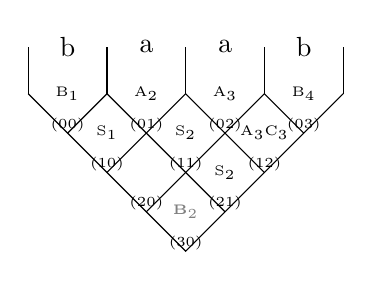
\begin{tikzpicture}[baseline]
					\newcommand{\myfontvars}[1]{
						\fontsize{4.9}{12}\selectfont{#1}
					}\newcommand{\myfontnumbering}[1]{
						\fontsize{2.5}{12}\selectfont{#1}
					}%Outer hull
					%Tip of the pyramid
					\coordinate (tip) at (2.0,-2.0);
					\foreach \i in {0,...,4} {
						\coordinate (\i) at (\i,0);
					}
					%Draw the left and right line of the pyramid pointing downwards
					\draw (0) -- (tip) -- (4);
					%Grid lines direction down-left to top-right
					\coordinate (dl1) at (0.5,-0.5);
					\coordinate (dl2) at (1.0,-1.0);
					\coordinate (dl3) at (1.5,-1.5);
					\draw (dl1) -- (1,0);
					\draw (dl2) -- (2,0);
					\draw (dl3) -- (3,0);
					%Grid lines direction down-right to top-left
					\coordinate (dr1) at (2.5,-1.5);
					\coordinate (dr2) at (3.0,-1.0);
					\coordinate (dr3) at (3.5,-0.5);
					\draw (dr1) -- (1,0);
					\draw (dr2) -- (2,0);
					\draw (dr3) -- (3,0);
					%Small lines at the top
					\coordinate (top0) at (0.0,0.0);
					\coordinate (top1) at (1.0,0.0);
					\coordinate (top2) at (2.0,0.0);
					\coordinate (top3) at (3.0,0.0);
					\coordinate (top4) at (4.0,0.0);
					\coordinate (topUpper0) at (0.0,0.6);
					\coordinate (topUpper1) at (1.0,0.6);
					\coordinate (topUpper2) at (2.0,0.6);
					\coordinate (topUpper3) at (3.0,0.6);
					\coordinate (topUpper4) at (4.0,0.6);
					\draw (top0) -- (topUpper0);
					\draw (top1) -- (topUpper1);
					\draw (top2) -- (topUpper2);
					\draw (top3) -- (topUpper3);
					\draw (top4) -- (topUpper4);
					%The string
					\coordinate (w0) at (0.5,0.6);
					\coordinate (w1) at (1.5,0.6);
					\coordinate (w2) at (2.5,0.6);
					\coordinate (w3) at (3.5,0.6);
					\node [] at (w0) {b};
					\node [] at (w1) {a};
					\node [] at (w2) {a};
					\node [] at (w3) {b};
					% Variables in the cells
					%cells00
					\coordinate (center00) at (0.5,0.0);
					\node [below=0.18cm] at (center00) {\myfontnumbering{$(00)$}};
					\node [] at (center00) {\myfontvars{B$_{1}$}};
					%cells01
					\coordinate (center01) at (1.5,0.0);
					\node [below=0.18cm] at (center01) {\myfontnumbering{$(01)$}};
					\node [] at (center01) {\myfontvars{A$_{2}$}};
					%cells02
					\coordinate (center02) at (2.5,0.0);
					\node [below=0.18cm] at (center02) {\myfontnumbering{$(02)$}};
					\node [] at (center02) {\myfontvars{A$_{3}$}};
					%cells03
					\coordinate (center03) at (3.5,0.0);
					\node [below=0.18cm] at (center03) {\myfontnumbering{$(03)$}};
					\node [] at (center03) {\myfontvars{B$_{4}$}};
					%cells10
					\coordinate (center10) at (1.0,-0.5);
					\node [below=0.18cm] at (center10) {\myfontnumbering{$(10)$}};
					\node [] at (center10) {\myfontvars{S$_{1}$}};
					%cells11
					\coordinate (center11) at (2.0,-0.5);
					\node [below=0.18cm] at (center11) {\myfontnumbering{$(11)$}};
					\node [] at (center11) {\myfontvars{S$_{2}$}};
					%cells12
					\coordinate (center12) at (3.0,-0.5);
					\node [below=0.18cm] at (center12) {\myfontnumbering{$(12)$}};
					\node [] at (center12) {\myfontvars{A$_{3}$C$_{3}$}};
					%cells20
					\coordinate (center20) at (1.5,-1.0);
					\node [below=0.18cm] at (center20) {\myfontnumbering{$(20)$}};
					%cells21
					\coordinate (center21) at (2.5,-1.0);
					\node [below=0.18cm] at (center21) {\myfontnumbering{$(21)$}};
					\node [] at (center21) {\myfontvars{S$_{2}$}};
					%cells30
					\coordinate (center30) at (2.0,-1.5);
					\node [below=0.18cm] at (center30) {\myfontnumbering{$(30)$}};
					\node [] at (center30) {\myfontvars{\textcolor{gray}{\textbf{B$_{2}$}}}};
					\end{tikzpicture}
				}	
			}
		}
	\end{minipage}
\end{figure}\\
Then the calculation of CellSet for $Cell_{3,0}$ results in $\{SA,~SC,~BS\}$, whereas $SA$ and $SC$ stem from $Cell_{1,0}$ together with $Cell_{1,2}$ and $BA$ is from $Cell_{0,0}$ together with $Cell_{2,1}$. Now if either one of the rules $lhse \rightarrow SA$, $lhse \rightarrow SC$ or  $lhse \rightarrow BS$ is added to the grammar, then $lhse\in Cell_{3,0}$. Here the rule  \textcolor{gray}{\textbf{B $\rightarrow$ SC}} has been added and now $(B,2)$ is element of $Cell_{3,0}$.\\

\noindent \textbf{Choose one xy from (xy,i) $\in$ RowSet uniform randomly with probability depending on row i \circled{E} :}\\
There is the set $RowSet \subseteq \{(xy,i)\ |\ x,y \in V \wedge i \in \mathbb{N} \}$ and one xy is chosen out of it as following:
Firstly the $RowSet$ is compressed, i.e. every tuple with the same $xy$ will be merged to its lowest $i$, as following: $RowSet = \{(AB,3),~(AB,1),~(AB,5),~... \}$ will become $RowSet = \{(AB,1),~... \}$. Afterwards all elements of $RowSet$ will be placed in the $RowMultiSet$ that  can contain multiple equivalent elements. Now each element of $RowMultiSet$ will be weighted according to their $i$. That means that elements like $(AB,1)$ will only occur one time though elements like $(BC,3)$ will occur three times and so on: $RowMultiSet = \{(AB,1),~(BC,3),~...\}$ becomes $RowMultiSet = \{(AB,1),~(BC,3),~(BC,3),~(BC,3),~...\}$. Now one element will be uniform randomly picked out of this weighted $RowMultiSet$ like $xy = BC$.\\

\noindent
\begin{figure} [h]
	\begin{minipage}{6in}
		\centering
		\raisebox{-0.5\height}{
		\begin{tabular}{l l}
			$RowSet = \{(AB,3),(AB,1),(AB,5),... \}$ & // compress \\
			$RowSet = \{(AB,1),... \}$ & // place into RowMultiSet \\
			$RowMultiSet = \{(AB,1),(BC,3),...\}$ & // weight elements \\
			$RowMultiSet = \{(AB,1),(BC,3),(BC,3),(BC,3),...\}$ & // pick element\\
			$xy = BC$
		\end{tabular} 
		} 		
	\end{minipage}
	\caption{Short example of the procedure E.}
	\label{DiceRollONlyCYKExample}
\end{figure}

\subsection{DiceRollOnlyCYK}
\noindent This is a naive way of generating grammars, which will be the lower boundary while comparing the algorithms. Each future algorithm should have a higher score than this algorithm or otherwise it would be worse, than simple dice rolling the distribution of terminals (Line \ref{diceRollOnlyA}) and compound variables (Line \ref{diceRollOnlyB}). \\

\noindent
\frame{
	\begin{algorithm}[H] %or another one check
		\caption{DiceRollOnlyCYK}
		\label{DiceRollOnlyCYK}
		\SetAlgoLined
		\KwIn{Word $w \in \Sigma^{*}$ }
		\KwOut{Set of productions $P$}
		$P = \emptyset$;~~\tcp{$P \subseteq V \times (V^{2} \cup \Sigma)$}
		$P = Distribute(\Sigma,\ V)$;  \circled{A}\\ \label{diceRollOnlyA}
		$P \cup Distribute(V^2,\ V)$;  \circled{B}\\ \label{diceRollOnlyB}
		\Return $P$\;
	\end{algorithm}
}
A terminal $\Sigma$ is distributed to at least one $lhse$, but a compound variable $V^2$ must not be distributed at all. This means that for each terminal of $\Sigma=\{a,b\}$ there exists at least one rule like $lhse\rightarrow a$ and $lhse\rightarrow b$ and for each possible compound variable $V^2=\{AA,~AB,~AC,~AS,~BB,~BC,~BS,~CC,$ $~CS,SS\}$ it is possible that only a smaller subset like $\{AA,~BA,~CC,~SC\}$ is distributed so that only rules like $lhse\rightarrow AA$, $lhse\rightarrow BA$, $lhse\rightarrow CC$ and $lhse\rightarrow SC$ exist.
\noindent
\begin{figure} [h]
	\begin{minipage}{6in}
		\centering
		\raisebox{-0.5\height}{
		\begin{tabular}{l}
				Grammar after Line 2:\\
				$C\rightarrow a$\\ 
				$B\rightarrow b$\\
				\\
			\end{tabular} 
		\begin{tabular}{l}
			Grammar after Line 3:\\
			$C\rightarrow BA~|~AA~|~a$\\ 
			$B\rightarrow b$ \\
			$S\rightarrow CC~|~SC$ 
		\end{tabular}
	} 		
	\end{minipage}
	\caption{Short example of Algorithm \ref{DiceRollOnlyCYK}.}
	\label{DiceRollONlyCYKExample}
\end{figure}
\subsection{BottomUpDiceRollVar1}
This algorithm uses the Bottom-Up approach (Chapter \ref{approaches}) whereby the parsing table is filled starting from the leaves in direction to the root node.\\
The basic idea behind this algorithm is to guide the choice of rules while distributing the compound variables $V^2$. In Algorithm \ref{DiceRollOnlyCYK} it can happen that the terminals are distributed to the variables $A$ and $B$ and Algorithm \ref{DiceRollOnlyCYK} completely discards this fact during the distribution of the compound variables. In a situation as seen below it can happen \\
\noindent
\begin{figure}[h]
	\begin{minipage}{6in}
		\centering
		\raisebox{-0.5\height}{
			\begin{tabular}{l}
				Grammar:\\
				$A\rightarrow a$\\
				$B \rightarrow b$\\ 
			\end{tabular} 
		}
		\hspace*{.2in}
		\raisebox{-0.5\height}{
			\resizebox{0.5\linewidth}{!}{
				\resizebox{\linewidth}{!}{
					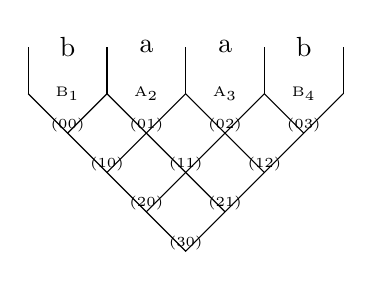
\begin{tikzpicture}[baseline]
					\newcommand{\myfontvars}[1]{
						\fontsize{4.9}{12}\selectfont{#1}
					}\newcommand{\myfontnumbering}[1]{
						\fontsize{2.5}{12}\selectfont{#1}
					}%Outer hull
					%Tip of the pyramid
					\coordinate (tip) at (2.0,-2.0);
					\foreach \i in {0,...,4} {
						\coordinate (\i) at (\i,0);
					}
					%Draw the left and right line of the pyramid pointing downwards
					\draw (0) -- (tip) -- (4);
					%Grid lines direction down-left to top-right
					\coordinate (dl1) at (0.5,-0.5);
					\coordinate (dl2) at (1.0,-1.0);
					\coordinate (dl3) at (1.5,-1.5);
					\draw (dl1) -- (1,0);
					\draw (dl2) -- (2,0);
					\draw (dl3) -- (3,0);
					%Grid lines direction down-right to top-left
					\coordinate (dr1) at (2.5,-1.5);
					\coordinate (dr2) at (3.0,-1.0);
					\coordinate (dr3) at (3.5,-0.5);
					\draw (dr1) -- (1,0);
					\draw (dr2) -- (2,0);
					\draw (dr3) -- (3,0);
					%Small lines at the top
					\coordinate (top0) at (0.0,0.0);
					\coordinate (top1) at (1.0,0.0);
					\coordinate (top2) at (2.0,0.0);
					\coordinate (top3) at (3.0,0.0);
					\coordinate (top4) at (4.0,0.0);
					\coordinate (topUpper0) at (0.0,0.6);
					\coordinate (topUpper1) at (1.0,0.6);
					\coordinate (topUpper2) at (2.0,0.6);
					\coordinate (topUpper3) at (3.0,0.6);
					\coordinate (topUpper4) at (4.0,0.6);
					\draw (top0) -- (topUpper0);
					\draw (top1) -- (topUpper1);
					\draw (top2) -- (topUpper2);
					\draw (top3) -- (topUpper3);
					\draw (top4) -- (topUpper4);
					%The string
					\coordinate (w0) at (0.5,0.6);
					\coordinate (w1) at (1.5,0.6);
					\coordinate (w2) at (2.5,0.6);
					\coordinate (w3) at (3.5,0.6);
					\node [] at (w0) {b};
					\node [] at (w1) {a};
					\node [] at (w2) {a};
					\node [] at (w3) {b};
					% Variables in the cells
					%cells00
					\coordinate (center00) at (0.5,0.0);
					\node [below=0.18cm] at (center00) {\myfontnumbering{$(00)$}};
					\node [] at (center00) {\myfontvars{B$_{1}$}};
					%cells01
					\coordinate (center01) at (1.5,0.0);
					\node [below=0.18cm] at (center01) {\myfontnumbering{$(01)$}};
					\node [] at (center01) {\myfontvars{A$_{2}$}};
					%cells02
					\coordinate (center02) at (2.5,0.0);
					\node [below=0.18cm] at (center02) {\myfontnumbering{$(02)$}};
					\node [] at (center02) {\myfontvars{A$_{3}$}};
					%cells03
					\coordinate (center03) at (3.5,0.0);
					\node [below=0.18cm] at (center03) {\myfontnumbering{$(03)$}};
					\node [] at (center03) {\myfontvars{B$_{4}$}};
					%cells10
					\coordinate (center10) at (1.0,-0.5);
					\node [below=0.18cm] at (center10) {\myfontnumbering{$(10)$}};
					%cells11
					\coordinate (center11) at (2.0,-0.5);
					\node [below=0.18cm] at (center11) {\myfontnumbering{$(11)$}};
					%cells12
					\coordinate (center12) at (3.0,-0.5);
					\node [below=0.18cm] at (center12) {\myfontnumbering{$(12)$}};
					%cells20
					\coordinate (center20) at (1.5,-1.0);
					\node [below=0.18cm] at (center20) {\myfontnumbering{$(20)$}};
					%cells21
					\coordinate (center21) at (2.5,-1.0);
					\node [below=0.18cm] at (center21) {\myfontnumbering{$(21)$}};
					%cells30
					\coordinate (center30) at (2.0,-1.5);
					\node [below=0.18cm] at (center30) {\myfontnumbering{$(30)$}};
					\end{tikzpicture}
				}	
			}
		}
	\end{minipage}
\end{figure}\\
that rules like $lhse \rightarrow CC$ or $lhse \rightarrow SC$ are added, that obviously not directly help to fill the parsing table and bloat the grammar with useless rules. More reasonably rules to add would be $lhse \rightarrow BA$, $lhse \rightarrow AA$ and $lhse \rightarrow AB$.\\
Algorithm \ref{BottomUpDiceRollVar1} takes this up: After distributing the terminals (Line \ref{var1A}) the updated parsing table (Line \ref{var1Update}) is always taken into consideration while choosing (Line \ref{var1E}) variable compounds and to finally add them (Line \ref{var1Add}). I.e. for each chosen cell a $CellSet$ is calculated, that only contains reasonably variable compounds. Now only variable compounds are added that directly help to fill the parsing table.\\

\noindent
\frame{
	\begin{algorithm}[H] %or another one check
		\caption{BottomUpDiceRollVar1}
		\label{BottomUpDiceRollVar1}
		\SetAlgoLined
		\KwIn{Word $w \in \Sigma^{*}$ }
		\KwOut{Set of productions $P$}
		$P = \emptyset$;~~\tcp{$P \subseteq V \times (V^{2} \cup \Sigma)$}
		$P = Distribute(\Sigma,\ V)$;  \circled{A}\\
		$Pyramid = CYK(G,\ w)$\label{stepii}\;
		\For{$i:=1\ \textbf{to}\ i_{max}$}{
			$J = \{0,~...~,~j_{max} -1\}$;~~\tcp{$J \subseteq \mathbb{N}$}
			$CellSet = \emptyset$;~~\tcp{$CellSet \subseteq V^2$} \label{var1A}
			\While{$|J|>0$}{
				$choose\ one\ j \in J\ uniform\ randomly$\label{chooseJ}\;
				$J = J \setminus \{j\} $\;
				$CellSet = CalculateSubsetForCell(Pyramid,\ i,\ j)$;  \circled{D} \label{var1E}\\
				$P \cup Distribute(CellSet,\ V)$;  \circled{B} \label{var1Add}\\
				$Pyramid = CYK(G,\ w)$\; \label{var1Update}
				\If{$stopping\ criteria~met$~\circled{C}}{
					\Return $P$\;
				}
			}
		}
		\Return $P$\;
		\footnotetext{
			\noindent Line \ref{stepii}: Fills the i=0 row of the pyramid.
			
			\noindent Line \ref{chooseJ}: A cell is only visited only once.
		}
	\end{algorithm}
}

\pagebreak
\subsection{BottomUpDiceRollVar2}
While examining the Algorithm \ref{BottomUpDiceRollVar1} via its log files [XXX] it can be seen that already a very small number of rules in the grammar is sufficient so that the stopping criteria \circled{C} is met \textendash~the cells that indirectly decide what rules to add are mostly from row one ($i=1$) and sometimes if at all from row two ($i=2$).\\ 
This again leads to another idea to introduce a row dependent $threshold_i$ (Line \ref{var2threshold}) that helps that more cells with $i\geq2$ are chosen \textendash~what possibly can lead to more diverse (= homogeneity criteria, see Chapter \ref{scoringModel}) grammars. The diversity, in context of Algorithm \ref{BottomUpDiceRollVar1}, is somewhat too restricted to the $lhse$s that have one of the terminals as its $rhse$. Most of the rules that are part of the grammar will contain one these $lhse$s. This is due to the basic idea of Algorithm \ref{BottomUpDiceRollVar1} but also due to the relatively small number of rules in the grammar. \\
Further diversification is achieved through the usage of \circled{E} (Line \ref{chooseVc}). Variable compounds that already have been used in a row with low index $i$ are at a disadvantage to be picked again as described in Algorithm \ref{CalculateSubsetForCell}.\\
As seen in Figure \ref{GoalofBetterDiversity} rules with the same $rhse = BA~and~AA$ have been added to the variables $B$ and $A$ in Grammar1. For Grammar2 instead the rule $B\rightarrow SS$ was added that contributes to a better diversity.
\noindent
\begin{figure} [h]
	\begin{minipage}{6in}
		\centering
		\raisebox{-0.5\height}{
			\begin{tabular}{l}
				Grammar0:\\
				$C\rightarrow BA~|~AA~|~a$\\ 
				$B\rightarrow b$ \\
				$S\rightarrow CC~|~SC$ 
			\end{tabular}
			\begin{tabular}{l}
				Grammar1:\\
				$C\rightarrow BA~|~AA~|~a$\\ 
				$B\rightarrow BA~|~AA~|~b$ \\
				$S\rightarrow BA~|~AA~|~CC~|~SC$ 
			\end{tabular}
			\begin{tabular}{l}
			Grammar2:\\
			$C\rightarrow BA~|~AA~|~a$\\ 
			$B\rightarrow SS~|~b$ \\
			$S\rightarrow CC~|~SC$ 
		\end{tabular}
		} 		
	\end{minipage}
	\caption{Goal of better diversity: Starting point is Grammar0. Grammar2 is of better diversity than Grammar1.}
	\label{GoalofBetterDiversity}
\end{figure}


\noindent
\frame{
	\begin{algorithm}[H] %or another one check
		\caption{BottomUpDiceRollVar2}
		\label{BottomUpDiceRollVar2}
		\SetAlgoLined
		\KwIn{Word $w \in \Sigma^{*}$ }
		\KwOut{Set of productions $P$}
		$P = \emptyset$;~~\tcp{$P \subseteq V \times (V^{2} \cup \Sigma)$}
		$RowSet = \emptyset$;~~\tcp{$RowSet \subseteq \{(xy,i)\ |\ x,y \in V \wedge i \in \mathbb{N} \}$}
		$P = Distribute(\Sigma,\ V)$;  \circled{A}\\
		$Pyramid = CYK(G,\ w)$ \label{stepii}\;
		\For{$i:=1\ \textbf{to}\ i_{max}$}{
			%$choose\ j\ uniform\ randomly\ in\ [0,\ j_{max}-i]  $\;
			\For{$j:=0\ \textbf{to}\ j_{max}-i$}{
				$RowSet \cup \{(xy,i)\ |\ xy \in CalculateSubsetForCell(Pyramid,\ i,\ j) $\circled{D}$\}$\label{rowSet}\;  
			}
			\While{$threshold_i\ not\ reached $}{ \label{var2threshold}
				$choose\ one~xy\ from\ (xy,\ i) \in RowSet~uniform\ randomly\ with$ $probability~depending~on~i $;\label{chooseVc} \circled{E}  \\
				$P \cup Distribute(xy,\ V) $; \circled{B}  \\
				$Pyramid = CYK(G,\ w)$\;
				\If{$stopping\ criteria~met$~\circled{C}}{
					\Return $P$\;
				}	
			}
		}
		\Return $P$\;
		\footnotetext{
			\noindent Line \ref{stepii}: Fills the i=0 row of the pyramid.
		}
	\end{algorithm}
}



\pagebreak
\subsection{SplitThenFill}

The idea here is to first distribute the terminals (Line \ref{splitThenStepii} of Algorithm \ref{SplitThenFill}) and then to uniform randomly generate a predefined structure of the derivation tree (Line \ref{splitThenFillTreeStart} of Algorithm \ref{splitThenStepii} and in general Algorithm \ref{SplitThenFillRecursion}) Top-Downwards and then again to fill the parsing table Bottom-Upwards accordingly to this derivation tree. The reason behind its name comes from the fact that only after completely generating the structure (splitting of the word in subwords) of the derivation tree then the rules are added to the grammar that allows further filling of the parsing table. \\
Every time before adding a new rule (Algorithm \ref{SplitThenFillRecursion} Line \ref{splitThenFillB}) the already available information regarding the other rules is used to determine if a new rule is needed to fill this node of the derivation tree (Line \ref{empty} of Algorithm \ref{SplitThenFillRecursion}).\\


\noindent
\frame{
	\begin{algorithm}[H] %or another one check
		\caption{SplitThenFill}
		\label{SplitThenFill}
		\SetAlgoLined
		\KwIn{Word $w \in \Sigma^{*}$}
		\KwOut{Set of productions $P$}
		$P = \emptyset$;~~\tcp{$P \subseteq V \times (V^{2} \cup \Sigma)$}
		$P = Distribute(\Sigma,\ V)$; \circled{A} \label{splitThenStepii}  \\		
		$Sol = (P_{Sol},~Cell_{i_{max},0})$;~~\tcp{$P_{Sol} \subseteq P~\wedge~ Cell_{i_{max},0} \in Pyramid$} \label{cell}
		$Sol = SplitThenFillRec(P,\ w,\ i_{max},\ 0)$\; \label{splitThenFillTreeStart}
		\Return $P_{Sol}$\;
		\footnotetext{
			\noindent Line \ref{splitThenStepii}: Fills the i=0 row of the pyramid.	
		}
	\end{algorithm}
}
\\
For this algorithm it is important to mention that while using \circled{B} (Line \ref{splitThenFillB} of Algorithm \ref{SplitThenFillRecursion}) a variable compound is added to at least one $lhse$. For every element of $Vc$ (Line \ref{splitThenFillVc} of Algorithm \ref{SplitThenFillRecursion}) there exists at least one rule $lhse \rightarrow vc$ with $vc \in Vc$.\\
The construction of the derivation tree for instance is done as following \textendash~each number represents the recursion depth of its subtree: 
\begin{center}
	\begin{figure} [h]
		\centering
	\resizebox{0.65\linewidth}{!}{
		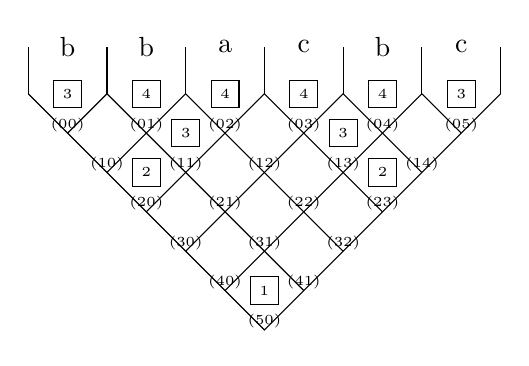
\begin{tikzpicture}[baseline]
		\newcommand{\myfontvars}[1]{
			\fontsize{4.9}{12}\selectfont{#1}
		}\newcommand{\myfontnumbering}[1]{
			\fontsize{2.5}{12}\selectfont{#1}
		}%Outer hull
		%Tip of the pyramid
		\coordinate (tip) at (3.0,-3.0);
		\foreach \i in {0,...,6} {
			\coordinate (\i) at (\i,0);
		}
		%Draw the left and right line of the pyramid pointing downwards
		\draw (0) -- (tip) -- (6);
		%Grid lines direction down-left to top-right
		\coordinate (dl1) at (0.5,-0.5);
		\coordinate (dl2) at (1.0,-1.0);
		\coordinate (dl3) at (1.5,-1.5);
		\coordinate (dl4) at (2.0,-2.0);
		\coordinate (dl5) at (2.5,-2.5);
		\draw (dl1) -- (1,0);
		\draw (dl2) -- (2,0);
		\draw (dl3) -- (3,0);
		\draw (dl4) -- (4,0);
		\draw (dl5) -- (5,0);
		%Grid lines direction down-right to top-left
		\coordinate (dr1) at (3.5,-2.5);
		\coordinate (dr2) at (4.0,-2.0);
		\coordinate (dr3) at (4.5,-1.5);
		\coordinate (dr4) at (5.0,-1.0);
		\coordinate (dr5) at (5.5,-0.5);
		\draw (dr1) -- (1,0);
		\draw (dr2) -- (2,0);
		\draw (dr3) -- (3,0);
		\draw (dr4) -- (4,0);
		\draw (dr5) -- (5,0);
		%Small lines at the top
		\coordinate (top0) at (0.0,0.0);
		\coordinate (top1) at (1.0,0.0);
		\coordinate (top2) at (2.0,0.0);
		\coordinate (top3) at (3.0,0.0);
		\coordinate (top4) at (4.0,0.0);
		\coordinate (top5) at (5.0,0.0);
		\coordinate (top6) at (6.0,0.0);
		\coordinate (topUpper0) at (0.0,0.6);
		\coordinate (topUpper1) at (1.0,0.6);
		\coordinate (topUpper2) at (2.0,0.6);
		\coordinate (topUpper3) at (3.0,0.6);
		\coordinate (topUpper4) at (4.0,0.6);
		\coordinate (topUpper5) at (5.0,0.6);
		\coordinate (topUpper6) at (6.0,0.6);
		\draw (top0) -- (topUpper0);
		\draw (top1) -- (topUpper1);
		\draw (top2) -- (topUpper2);
		\draw (top3) -- (topUpper3);
		\draw (top4) -- (topUpper4);
		\draw (top5) -- (topUpper5);
		\draw (top6) -- (topUpper6);
		%The string
		\coordinate (w0) at (0.5,0.6);
		\coordinate (w1) at (1.5,0.6);
		\coordinate (w2) at (2.5,0.6);
		\coordinate (w3) at (3.5,0.6);
		\coordinate (w4) at (4.5,0.6);
		\coordinate (w5) at (5.5,0.6);
		\node [] at (w0) {b};
		\node [] at (w1) {b};
		\node [] at (w2) {a};
		\node [] at (w3) {c};
		\node [] at (w4) {b};
		\node [] at (w5) {c};
		% Variables in the cells
		%cells00
		\coordinate (center00) at (0.5,0.0);
		\node [below=0.18cm] at (center00) {\myfontnumbering{$(00)$}};
		\node [] at (center00) [minimum height=0.25cm,minimum width=0.25cm,draw] {\tiny{3}};
		%cells01
		\coordinate (center01) at (1.5,0.0);
		\node [below=0.18cm] at (center01) {\myfontnumbering{$(01)$}};
		\node [] at (center01) [minimum height=0.25cm,minimum width=0.25cm,draw] {\tiny{4}};
		%cells02
		\coordinate (center02) at (2.5,0.0);
		\node [below=0.18cm] at (center02) {\myfontnumbering{$(02)$}};
		\node [] at (center02) [minimum height=0.25cm,minimum width=0.25cm,draw] {\tiny{4}};
		%cells03
		\coordinate (center03) at (3.5,0.0);
		\node [below=0.18cm] at (center03) {\myfontnumbering{$(03)$}};
		\node [] at (center03) [minimum height=0.25cm,minimum width=0.25cm,draw] {\tiny{4}};
		%cells04
		\coordinate (center04) at (4.5,0.0);
		\node [below=0.18cm] at (center04) {\myfontnumbering{$(04)$}};
		\node [] at (center04) [minimum height=0.25cm,minimum width=0.25cm,draw] {\tiny{4}};
		%cells05
		\coordinate (center05) at (5.5,0.0);
		\node [below=0.18cm] at (center05) {\myfontnumbering{$(05)$}};
		\node [] at (center05) [minimum height=0.25cm,minimum width=0.25cm,draw] {\tiny{3}};
		%cells10
		\coordinate (center10) at (1.0,-0.5);
		\node [below=0.18cm] at (center10) {\myfontnumbering{$(10)$}};
		%cells11
		\coordinate (center11) at (2.0,-0.5);
		\node [below=0.18cm] at (center11) {\myfontnumbering{$(11)$}};
		\node [] at (center11) [minimum height=0.25cm,minimum width=0.25cm,draw] {\tiny{3}};
		%cells12
		\coordinate (center12) at (3.0,-0.5);
		\node [below=0.18cm] at (center12) {\myfontnumbering{$(12)$}};
		%cells13
		\coordinate (center13) at (4.0,-0.5);
		\node [below=0.18cm] at (center13) {\myfontnumbering{$(13)$}};
		\node [] at (center13) [minimum height=0.25cm,minimum width=0.25cm,draw] {\tiny{3}};
		%cells14
		\coordinate (center14) at (5.0,-0.5);
		\node [below=0.18cm] at (center14) {\myfontnumbering{$(14)$}};
		%cells20
		\coordinate (center20) at (1.5,-1.0);
		\node [below=0.18cm] at (center20) {\myfontnumbering{$(20)$}};
		\node [] at (center20) [minimum height=0.25cm,minimum width=0.25cm,draw] {\tiny{2}};
		%cells21
		\coordinate (center21) at (2.5,-1.0);
		\node [below=0.18cm] at (center21) {\myfontnumbering{$(21)$}};
		%cells22
		\coordinate (center22) at (3.5,-1.0);
		\node [below=0.18cm] at (center22) {\myfontnumbering{$(22)$}};
		%cells23
		\coordinate (center23) at (4.5,-1.0);
		\node [below=0.18cm] at (center23) {\myfontnumbering{$(23)$}};
		\node [] at (center23) [minimum height=0.25cm,minimum width=0.25cm,draw] {\tiny{2}};
		%cells30
		\coordinate (center30) at (2.0,-1.5);
		\node [below=0.18cm] at (center30) {\myfontnumbering{$(30)$}};
		%cells31
		\coordinate (center31) at (3.0,-1.5);
		\node [below=0.18cm] at (center31) {\myfontnumbering{$(31)$}};
		%cells32
		\coordinate (center32) at (4.0,-1.5);
		\node [below=0.18cm] at (center32) {\myfontnumbering{$(32)$}};
		%cells40
		\coordinate (center40) at (2.5,-2.0);
		\node [below=0.18cm] at (center40) {\myfontnumbering{$(40)$}};
		%cells41
		\coordinate (center41) at (3.5,-2.0);
		\node [below=0.18cm] at (center41) {\myfontnumbering{$(41)$}};
		%cells50
		\coordinate (center50) at (3.0,-2.5);
		\node [below=0.18cm] at (center50) {\myfontnumbering{$(50)$}};
		\node [] at (center50) [minimum height=0.25cm,minimum width=0.25cm,draw] {\tiny{1}};
		\end{tikzpicture}
	}
	\label{treeStruct}
	\caption{Example derivation tree structure.}
	\end{figure}
\end{center}

\noindent
\frame{
	\begin{algorithm}[H] %or another one check
		\caption{SplitThenFillRec}
		\label{SplitThenFillRecursion}
		\SetAlgoLined
		\KwIn{$P_{in} \subseteq V \times (V^{2} \cup \Sigma),\ w \in \Sigma^{*},\ i,j \in \mathbb{N}$ }
		\KwOut{$(P,~Cell_{i,j})$}
		$P =  P_{in}$\;
		\If{$i=0$}{
			\Return $(P,\ Cell_{i,j})$\label{row0}\;
		}	
		$choose\ one\ m\ uniform\ randomly\ in\ [j+1,\ j+i]$\;
		$(P,\ Cell_l) = SplitThenFillRec(P,\ w,\ (m-j-1),\ j)$\label{left}\;
		$(P,\ Cell_r) = SplitThenFillRec(P,\ w,\ (j+i-m),\ m)$\label{right}\;
		$Pyramid = CYK(G,\ w)$\label{cyk}\;
		\If{$stopping\ criteria~met$~\circled{C}}{
			\Return $(P,\ Cell_{i,j})$\;
		}
		\If{$Cell_{i,j} = \emptyset$}{ \label{empty}
			$VarComp = uniform\ random\ subset\ from\ \{vc\ |\ v \in Cell_l\ \wedge\ c \in Cell_r\} ~with~|VarComp| \geq 1$\; \label{splitThenFillVc}
			$P \cup Distribute(VarComp,\ V) $; \circled{B} \label{splitThenFillB}  \\
		}
		
		\Return $(P,\ Cell_{i,j})$\;
	\end{algorithm}
}
The same example tree structure is used as seen in Figure \ref{treeStruct}.

\noindent
\begin{figure} [h]
	\begin{minipage}{6in}
		\centering
		\begin{tabular}{l}
			Grammar:\\
			$A \rightarrow a$\\
			$B \rightarrow b$\\ 
			$C \rightarrow c$\\
			$S \rightarrow $\\ 
		\end{tabular} 
		\resizebox{0.7\linewidth}{!}{
			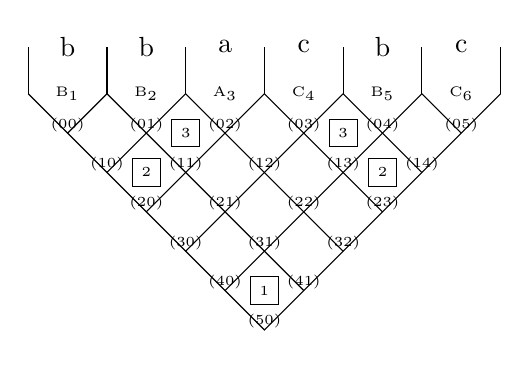
\begin{tikzpicture}[baseline]
			\newcommand{\myfontvars}[1]{
				\fontsize{4.9}{12}\selectfont{#1}
			}\newcommand{\myfontnumbering}[1]{
				\fontsize{2.5}{12}\selectfont{#1}
			}%Outer hull
			%Tip of the pyramid
			\coordinate (tip) at (3.0,-3.0);
			\foreach \i in {0,...,6} {
				\coordinate (\i) at (\i,0);
			}
			%Draw the left and right line of the pyramid pointing downwards
			\draw (0) -- (tip) -- (6);
			%Grid lines direction down-left to top-right
			\coordinate (dl1) at (0.5,-0.5);
			\coordinate (dl2) at (1.0,-1.0);
			\coordinate (dl3) at (1.5,-1.5);
			\coordinate (dl4) at (2.0,-2.0);
			\coordinate (dl5) at (2.5,-2.5);
			\draw (dl1) -- (1,0);
			\draw (dl2) -- (2,0);
			\draw (dl3) -- (3,0);
			\draw (dl4) -- (4,0);
			\draw (dl5) -- (5,0);
			%Grid lines direction down-right to top-left
			\coordinate (dr1) at (3.5,-2.5);
			\coordinate (dr2) at (4.0,-2.0);
			\coordinate (dr3) at (4.5,-1.5);
			\coordinate (dr4) at (5.0,-1.0);
			\coordinate (dr5) at (5.5,-0.5);
			\draw (dr1) -- (1,0);
			\draw (dr2) -- (2,0);
			\draw (dr3) -- (3,0);
			\draw (dr4) -- (4,0);
			\draw (dr5) -- (5,0);
			%Small lines at the top
			\coordinate (top0) at (0.0,0.0);
			\coordinate (top1) at (1.0,0.0);
			\coordinate (top2) at (2.0,0.0);
			\coordinate (top3) at (3.0,0.0);
			\coordinate (top4) at (4.0,0.0);
			\coordinate (top5) at (5.0,0.0);
			\coordinate (top6) at (6.0,0.0);
			\coordinate (topUpper0) at (0.0,0.6);
			\coordinate (topUpper1) at (1.0,0.6);
			\coordinate (topUpper2) at (2.0,0.6);
			\coordinate (topUpper3) at (3.0,0.6);
			\coordinate (topUpper4) at (4.0,0.6);
			\coordinate (topUpper5) at (5.0,0.6);
			\coordinate (topUpper6) at (6.0,0.6);
			\draw (top0) -- (topUpper0);
			\draw (top1) -- (topUpper1);
			\draw (top2) -- (topUpper2);
			\draw (top3) -- (topUpper3);
			\draw (top4) -- (topUpper4);
			\draw (top5) -- (topUpper5);
			\draw (top6) -- (topUpper6);
			%The string
			\coordinate (w0) at (0.5,0.6);
			\coordinate (w1) at (1.5,0.6);
			\coordinate (w2) at (2.5,0.6);
			\coordinate (w3) at (3.5,0.6);
			\coordinate (w4) at (4.5,0.6);
			\coordinate (w5) at (5.5,0.6);
			\node [] at (w0) {b};
			\node [] at (w1) {b};
			\node [] at (w2) {a};
			\node [] at (w3) {c};
			\node [] at (w4) {b};
			\node [] at (w5) {c};
			% Variables in the cells
			%cells00
			\coordinate (center00) at (0.5,0.0);
			\node [below=0.18cm] at (center00) {\myfontnumbering{$(00)$}};
			\node [] at (center00) {\myfontvars{B$_{1}$}};
			%cells01
			\coordinate (center01) at (1.5,0.0);
			\node [below=0.18cm] at (center01) {\myfontnumbering{$(01)$}};
			\node [] at (center01) {\myfontvars{B$_{2}$}};
			%cells02
			\coordinate (center02) at (2.5,0.0);
			\node [below=0.18cm] at (center02) {\myfontnumbering{$(02)$}};
			\node [] at (center02) {\myfontvars{A$_{3}$}};
			%cells03
			\coordinate (center03) at (3.5,0.0);
			\node [below=0.18cm] at (center03) {\myfontnumbering{$(03)$}};
			\node [] at (center03) {\myfontvars{C$_{4}$}};
			%cells04
			\coordinate (center04) at (4.5,0.0);
			\node [below=0.18cm] at (center04) {\myfontnumbering{$(04)$}};
			\node [] at (center04) {\myfontvars{B$_{5}$}};
			%cells05
			\coordinate (center05) at (5.5,0.0);
			\node [below=0.18cm] at (center05) {\myfontnumbering{$(05)$}};
			\node [] at (center05) {\myfontvars{C$_{6}$}};
			%cells10
			\coordinate (center10) at (1.0,-0.5);
			\node [below=0.18cm] at (center10) {\myfontnumbering{$(10)$}};
			%cells11
			\coordinate (center11) at (2.0,-0.5);
			\node [below=0.18cm] at (center11) {\myfontnumbering{$(11)$}};
			\node [] at (center11) [minimum height=0.25cm,minimum width=0.25cm,draw] {\tiny{3}};
			%cells12
			\coordinate (center12) at (3.0,-0.5);
			\node [below=0.18cm] at (center12) {\myfontnumbering{$(12)$}};
			%cells13
			\coordinate (center13) at (4.0,-0.5);
			\node [below=0.18cm] at (center13) {\myfontnumbering{$(13)$}};
			\node [] at (center13) [minimum height=0.25cm,minimum width=0.25cm,draw] {\tiny{3}};
			%cells14
			\coordinate (center14) at (5.0,-0.5);
			\node [below=0.18cm] at (center14) {\myfontnumbering{$(14)$}};
			%cells20
			\coordinate (center20) at (1.5,-1.0);
			\node [below=0.18cm] at (center20) {\myfontnumbering{$(20)$}};
			\node [] at (center20) [minimum height=0.25cm,minimum width=0.25cm,draw] {\tiny{2}};
			%cells21
			\coordinate (center21) at (2.5,-1.0);
			\node [below=0.18cm] at (center21) {\myfontnumbering{$(21)$}};
			%cells22
			\coordinate (center22) at (3.5,-1.0);
			\node [below=0.18cm] at (center22) {\myfontnumbering{$(22)$}};
			%cells23
			\coordinate (center23) at (4.5,-1.0);
			\node [below=0.18cm] at (center23) {\myfontnumbering{$(23)$}};
			\node [] at (center23) [minimum height=0.25cm,minimum width=0.25cm,draw] {\tiny{2}};
			%cells30
			\coordinate (center30) at (2.0,-1.5);
			\node [below=0.18cm] at (center30) {\myfontnumbering{$(30)$}};
			%cells31
			\coordinate (center31) at (3.0,-1.5);
			\node [below=0.18cm] at (center31) {\myfontnumbering{$(31)$}};
			%cells32
			\coordinate (center32) at (4.0,-1.5);
			\node [below=0.18cm] at (center32) {\myfontnumbering{$(32)$}};
			%cells40
			\coordinate (center40) at (2.5,-2.0);
			\node [below=0.18cm] at (center40) {\myfontnumbering{$(40)$}};
			%cells41
			\coordinate (center41) at (3.5,-2.0);
			\node [below=0.18cm] at (center41) {\myfontnumbering{$(41)$}};
			%cells50
			\coordinate (center50) at (3.0,-2.5);
			\node [below=0.18cm] at (center50) {\myfontnumbering{$(50)$}};
			\node [] at (center50) [minimum height=0.25cm,minimum width=0.25cm,draw] {\tiny{1}};
			\end{tikzpicture}
		}
	\end{minipage}
	\caption{Illustration of Algorithm \ref{SplitThenFill} part 1.}
	\label{IllustrationAlgorithmSplitThenFillPart1}
\end{figure}

\noindent After adding the terminals to the grammar (Line \ref{splitThenStepii} in Algorithm \ref{SplitThenFill}) now one must take on the recursion step at $Cell_{1,1}$. Now $Cell_l=\{B_2\}$ and $Cell_r=\{A_3\}$ and therefore $Vc={BA}$. Now adding the rule $S \rightarrow BA$ leads to the following changes: 

\noindent
\begin{figure} [h]
	\begin{minipage}{6in}
		\centering
		\begin{tabular}{l}
			Grammar:\\
			$A \rightarrow a$\\
			$B \rightarrow b$\\ 
			$C \rightarrow c$\\
			$S \rightarrow BA$\\ 
		\end{tabular} 
		\resizebox{0.7\linewidth}{!}{
			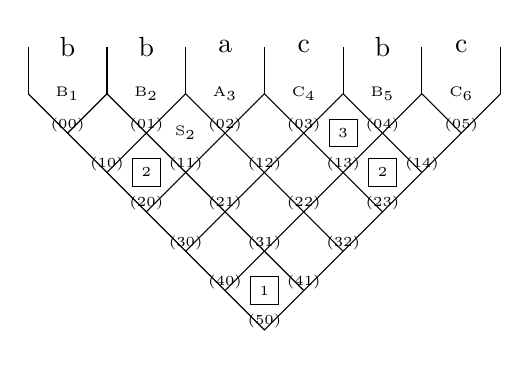
\begin{tikzpicture}[baseline]
			\newcommand{\myfontvars}[1]{
				\fontsize{4.9}{12}\selectfont{#1}
			}\newcommand{\myfontnumbering}[1]{
				\fontsize{2.5}{12}\selectfont{#1}
			}%Outer hull
			%Tip of the pyramid
			\coordinate (tip) at (3.0,-3.0);
			\foreach \i in {0,...,6} {
				\coordinate (\i) at (\i,0);
			}
			%Draw the left and right line of the pyramid pointing downwards
			\draw (0) -- (tip) -- (6);
			%Grid lines direction down-left to top-right
			\coordinate (dl1) at (0.5,-0.5);
			\coordinate (dl2) at (1.0,-1.0);
			\coordinate (dl3) at (1.5,-1.5);
			\coordinate (dl4) at (2.0,-2.0);
			\coordinate (dl5) at (2.5,-2.5);
			\draw (dl1) -- (1,0);
			\draw (dl2) -- (2,0);
			\draw (dl3) -- (3,0);
			\draw (dl4) -- (4,0);
			\draw (dl5) -- (5,0);
			%Grid lines direction down-right to top-left
			\coordinate (dr1) at (3.5,-2.5);
			\coordinate (dr2) at (4.0,-2.0);
			\coordinate (dr3) at (4.5,-1.5);
			\coordinate (dr4) at (5.0,-1.0);
			\coordinate (dr5) at (5.5,-0.5);
			\draw (dr1) -- (1,0);
			\draw (dr2) -- (2,0);
			\draw (dr3) -- (3,0);
			\draw (dr4) -- (4,0);
			\draw (dr5) -- (5,0);
			%Small lines at the top
			\coordinate (top0) at (0.0,0.0);
			\coordinate (top1) at (1.0,0.0);
			\coordinate (top2) at (2.0,0.0);
			\coordinate (top3) at (3.0,0.0);
			\coordinate (top4) at (4.0,0.0);
			\coordinate (top5) at (5.0,0.0);
			\coordinate (top6) at (6.0,0.0);
			\coordinate (topUpper0) at (0.0,0.6);
			\coordinate (topUpper1) at (1.0,0.6);
			\coordinate (topUpper2) at (2.0,0.6);
			\coordinate (topUpper3) at (3.0,0.6);
			\coordinate (topUpper4) at (4.0,0.6);
			\coordinate (topUpper5) at (5.0,0.6);
			\coordinate (topUpper6) at (6.0,0.6);
			\draw (top0) -- (topUpper0);
			\draw (top1) -- (topUpper1);
			\draw (top2) -- (topUpper2);
			\draw (top3) -- (topUpper3);
			\draw (top4) -- (topUpper4);
			\draw (top5) -- (topUpper5);
			\draw (top6) -- (topUpper6);
			%The string
			\coordinate (w0) at (0.5,0.6);
			\coordinate (w1) at (1.5,0.6);
			\coordinate (w2) at (2.5,0.6);
			\coordinate (w3) at (3.5,0.6);
			\coordinate (w4) at (4.5,0.6);
			\coordinate (w5) at (5.5,0.6);
			\node [] at (w0) {b};
			\node [] at (w1) {b};
			\node [] at (w2) {a};
			\node [] at (w3) {c};
			\node [] at (w4) {b};
			\node [] at (w5) {c};
			% Variables in the cells
			%cells00
			\coordinate (center00) at (0.5,0.0);
			\node [below=0.18cm] at (center00) {\myfontnumbering{$(00)$}};
			\node [] at (center00) {\myfontvars{B$_{1}$}};
			%cells01
			\coordinate (center01) at (1.5,0.0);
			\node [below=0.18cm] at (center01) {\myfontnumbering{$(01)$}};
			\node [] at (center01) {\myfontvars{B$_{2}$}};
			%cells02
			\coordinate (center02) at (2.5,0.0);
			\node [below=0.18cm] at (center02) {\myfontnumbering{$(02)$}};
			\node [] at (center02) {\myfontvars{A$_{3}$}};
			%cells03
			\coordinate (center03) at (3.5,0.0);
			\node [below=0.18cm] at (center03) {\myfontnumbering{$(03)$}};
			\node [] at (center03) {\myfontvars{C$_{4}$}};
			%cells04
			\coordinate (center04) at (4.5,0.0);
			\node [below=0.18cm] at (center04) {\myfontnumbering{$(04)$}};
			\node [] at (center04) {\myfontvars{B$_{5}$}};
			%cells05
			\coordinate (center05) at (5.5,0.0);
			\node [below=0.18cm] at (center05) {\myfontnumbering{$(05)$}};
			\node [] at (center05) {\myfontvars{C$_{6}$}};
			%cells10
			\coordinate (center10) at (1.0,-0.5);
			\node [below=0.18cm] at (center10) {\myfontnumbering{$(10)$}};
			%cells11
			\coordinate (center11) at (2.0,-0.5);
			\node [below=0.18cm] at (center11) {\myfontnumbering{$(11)$}};
			\node [] at (center11) {\myfontvars{S$_{2}$}};
			%cells12
			\coordinate (center12) at (3.0,-0.5);
			\node [below=0.18cm] at (center12) {\myfontnumbering{$(12)$}};
			%cells13
			\coordinate (center13) at (4.0,-0.5);
			\node [below=0.18cm] at (center13) {\myfontnumbering{$(13)$}};
			\node [] at (center13) [minimum height=0.25cm,minimum width=0.25cm,draw] {\tiny{3}};
			%cells14
			\coordinate (center14) at (5.0,-0.5);
			\node [below=0.18cm] at (center14) {\myfontnumbering{$(14)$}};
			%cells20
			\coordinate (center20) at (1.5,-1.0);
			\node [below=0.18cm] at (center20) {\myfontnumbering{$(20)$}};
			\node [] at (center20) [minimum height=0.25cm,minimum width=0.25cm,draw] {\tiny{2}};
			%cells21
			\coordinate (center21) at (2.5,-1.0);
			\node [below=0.18cm] at (center21) {\myfontnumbering{$(21)$}};
			%cells22
			\coordinate (center22) at (3.5,-1.0);
			\node [below=0.18cm] at (center22) {\myfontnumbering{$(22)$}};
			%cells23
			\coordinate (center23) at (4.5,-1.0);
			\node [below=0.18cm] at (center23) {\myfontnumbering{$(23)$}};
			\node [] at (center23) [minimum height=0.25cm,minimum width=0.25cm,draw] {\tiny{2}};
			%cells30
			\coordinate (center30) at (2.0,-1.5);
			\node [below=0.18cm] at (center30) {\myfontnumbering{$(30)$}};
			%cells31
			\coordinate (center31) at (3.0,-1.5);
			\node [below=0.18cm] at (center31) {\myfontnumbering{$(31)$}};
			%cells32
			\coordinate (center32) at (4.0,-1.5);
			\node [below=0.18cm] at (center32) {\myfontnumbering{$(32)$}};
			%cells40
			\coordinate (center40) at (2.5,-2.0);
			\node [below=0.18cm] at (center40) {\myfontnumbering{$(40)$}};
			%cells41
			\coordinate (center41) at (3.5,-2.0);
			\node [below=0.18cm] at (center41) {\myfontnumbering{$(41)$}};
			%cells50
			\coordinate (center50) at (3.0,-2.5);
			\node [below=0.18cm] at (center50) {\myfontnumbering{$(50)$}};
			\node [] at (center50) [minimum height=0.25cm,minimum width=0.25cm,draw] {\tiny{1}};
			\end{tikzpicture}
		}
	\end{minipage}
	\caption{Illustration of Algorithm \ref{SplitThenFill} part 2.}
	\label{IllustrationAlgorithmSplitThenFillPart2}
\end{figure}\\
\noindent The next recursion step happens in $Cell_{2,0}$. Now $Cell_l=\{B_1\}$ and $Cell_r=\{S_2\}$. Analogously the rule $A\rightarrow BS$ is added to the grammar:

\noindent
\begin{figure} [h]
	\begin{minipage}{6in}
		\centering
		\begin{tabular}{l}
			Grammar:\\
			$A \rightarrow BS~|~a$\\
			$B \rightarrow b$\\ 
			$C \rightarrow c$\\
			$S \rightarrow BA$\\ 
		\end{tabular} 
		\resizebox{0.7\linewidth}{!}{
			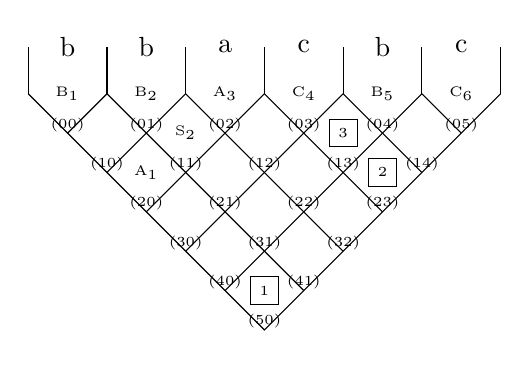
\begin{tikzpicture}[baseline]
			\newcommand{\myfontvars}[1]{
				\fontsize{4.9}{12}\selectfont{#1}
			}\newcommand{\myfontnumbering}[1]{
				\fontsize{2.5}{12}\selectfont{#1}
			}%Outer hull
			%Tip of the pyramid
			\coordinate (tip) at (3.0,-3.0);
			\foreach \i in {0,...,6} {
				\coordinate (\i) at (\i,0);
			}
			%Draw the left and right line of the pyramid pointing downwards
			\draw (0) -- (tip) -- (6);
			%Grid lines direction down-left to top-right
			\coordinate (dl1) at (0.5,-0.5);
			\coordinate (dl2) at (1.0,-1.0);
			\coordinate (dl3) at (1.5,-1.5);
			\coordinate (dl4) at (2.0,-2.0);
			\coordinate (dl5) at (2.5,-2.5);
			\draw (dl1) -- (1,0);
			\draw (dl2) -- (2,0);
			\draw (dl3) -- (3,0);
			\draw (dl4) -- (4,0);
			\draw (dl5) -- (5,0);
			%Grid lines direction down-right to top-left
			\coordinate (dr1) at (3.5,-2.5);
			\coordinate (dr2) at (4.0,-2.0);
			\coordinate (dr3) at (4.5,-1.5);
			\coordinate (dr4) at (5.0,-1.0);
			\coordinate (dr5) at (5.5,-0.5);
			\draw (dr1) -- (1,0);
			\draw (dr2) -- (2,0);
			\draw (dr3) -- (3,0);
			\draw (dr4) -- (4,0);
			\draw (dr5) -- (5,0);
			%Small lines at the top
			\coordinate (top0) at (0.0,0.0);
			\coordinate (top1) at (1.0,0.0);
			\coordinate (top2) at (2.0,0.0);
			\coordinate (top3) at (3.0,0.0);
			\coordinate (top4) at (4.0,0.0);
			\coordinate (top5) at (5.0,0.0);
			\coordinate (top6) at (6.0,0.0);
			\coordinate (topUpper0) at (0.0,0.6);
			\coordinate (topUpper1) at (1.0,0.6);
			\coordinate (topUpper2) at (2.0,0.6);
			\coordinate (topUpper3) at (3.0,0.6);
			\coordinate (topUpper4) at (4.0,0.6);
			\coordinate (topUpper5) at (5.0,0.6);
			\coordinate (topUpper6) at (6.0,0.6);
			\draw (top0) -- (topUpper0);
			\draw (top1) -- (topUpper1);
			\draw (top2) -- (topUpper2);
			\draw (top3) -- (topUpper3);
			\draw (top4) -- (topUpper4);
			\draw (top5) -- (topUpper5);
			\draw (top6) -- (topUpper6);
			%The string
			\coordinate (w0) at (0.5,0.6);
			\coordinate (w1) at (1.5,0.6);
			\coordinate (w2) at (2.5,0.6);
			\coordinate (w3) at (3.5,0.6);
			\coordinate (w4) at (4.5,0.6);
			\coordinate (w5) at (5.5,0.6);
			\node [] at (w0) {b};
			\node [] at (w1) {b};
			\node [] at (w2) {a};
			\node [] at (w3) {c};
			\node [] at (w4) {b};
			\node [] at (w5) {c};
			% Variables in the cells
			%cells00
			\coordinate (center00) at (0.5,0.0);
			\node [below=0.18cm] at (center00) {\myfontnumbering{$(00)$}};
			\node [] at (center00) {\myfontvars{B$_{1}$}};
			%cells01
			\coordinate (center01) at (1.5,0.0);
			\node [below=0.18cm] at (center01) {\myfontnumbering{$(01)$}};
			\node [] at (center01) {\myfontvars{B$_{2}$}};
			%cells02
			\coordinate (center02) at (2.5,0.0);
			\node [below=0.18cm] at (center02) {\myfontnumbering{$(02)$}};
			\node [] at (center02) {\myfontvars{A$_{3}$}};
			%cells03
			\coordinate (center03) at (3.5,0.0);
			\node [below=0.18cm] at (center03) {\myfontnumbering{$(03)$}};
			\node [] at (center03) {\myfontvars{C$_{4}$}};
			%cells04
			\coordinate (center04) at (4.5,0.0);
			\node [below=0.18cm] at (center04) {\myfontnumbering{$(04)$}};
			\node [] at (center04) {\myfontvars{B$_{5}$}};
			%cells05
			\coordinate (center05) at (5.5,0.0);
			\node [below=0.18cm] at (center05) {\myfontnumbering{$(05)$}};
			\node [] at (center05) {\myfontvars{C$_{6}$}};
			%cells10
			\coordinate (center10) at (1.0,-0.5);
			\node [below=0.18cm] at (center10) {\myfontnumbering{$(10)$}};
			%cells11
			\coordinate (center11) at (2.0,-0.5);
			\node [below=0.18cm] at (center11) {\myfontnumbering{$(11)$}};
			\node [] at (center11) {\myfontvars{S$_{2}$}};
			%cells12
			\coordinate (center12) at (3.0,-0.5);
			\node [below=0.18cm] at (center12) {\myfontnumbering{$(12)$}};
			%cells13
			\coordinate (center13) at (4.0,-0.5);
			\node [below=0.18cm] at (center13) {\myfontnumbering{$(13)$}};
			\node [] at (center13) [minimum height=0.25cm,minimum width=0.25cm,draw] {\tiny{3}};
			%cells14
			\coordinate (center14) at (5.0,-0.5);
			\node [below=0.18cm] at (center14) {\myfontnumbering{$(14)$}};
			%cells20
			\coordinate (center20) at (1.5,-1.0);
			\node [below=0.18cm] at (center20) {\myfontnumbering{$(20)$}};
			\node [] at (center20) {\myfontvars{A$_{1}$}};
			%cells21
			\coordinate (center21) at (2.5,-1.0);
			\node [below=0.18cm] at (center21) {\myfontnumbering{$(21)$}};
			%cells22
			\coordinate (center22) at (3.5,-1.0);
			\node [below=0.18cm] at (center22) {\myfontnumbering{$(22)$}};
			%cells23
			\coordinate (center23) at (4.5,-1.0);
			\node [below=0.18cm] at (center23) {\myfontnumbering{$(23)$}};
			\node [] at (center23) [minimum height=0.25cm,minimum width=0.25cm,draw] {\tiny{2}};
			%cells30
			\coordinate (center30) at (2.0,-1.5);
			\node [below=0.18cm] at (center30) {\myfontnumbering{$(30)$}};
			%cells31
			\coordinate (center31) at (3.0,-1.5);
			\node [below=0.18cm] at (center31) {\myfontnumbering{$(31)$}};
			%cells32
			\coordinate (center32) at (4.0,-1.5);
			\node [below=0.18cm] at (center32) {\myfontnumbering{$(32)$}};
			%cells40
			\coordinate (center40) at (2.5,-2.0);
			\node [below=0.18cm] at (center40) {\myfontnumbering{$(40)$}};
			%cells41
			\coordinate (center41) at (3.5,-2.0);
			\node [below=0.18cm] at (center41) {\myfontnumbering{$(41)$}};
			%cells50
			\coordinate (center50) at (3.0,-2.5);
			\node [below=0.18cm] at (center50) {\myfontnumbering{$(50)$}};
			\node [] at (center50) [minimum height=0.25cm,minimum width=0.25cm,draw] {\tiny{1}};
			\end{tikzpicture}
		}
	\end{minipage}
	\caption{Illustration of Algorithm \ref{SplitThenFill} part 3.}
	\label{IllustrationAlgorithmSplitThenFillPart3}
\end{figure}\\

\noindent
\begin{figure} [h]
	\begin{minipage}{6in}
		\centering
		\begin{tabular}{l}
			Grammar:\\
			$A \rightarrow BS~|~a$\\
			$B \rightarrow CB~|~b$\\ 
			$C \rightarrow c$\\
			$S \rightarrow BA$\\ 
		\end{tabular} 
		\resizebox{0.7\linewidth}{!}{
			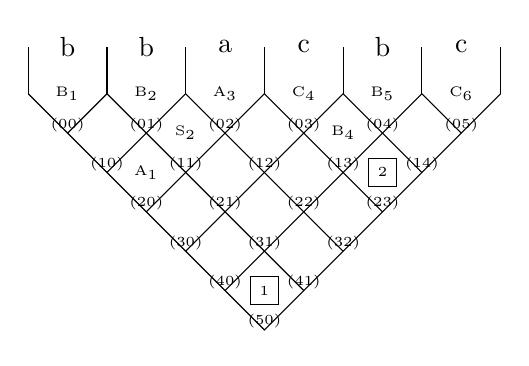
\begin{tikzpicture}[baseline]
			\newcommand{\myfontvars}[1]{
				\fontsize{4.9}{12}\selectfont{#1}
			}\newcommand{\myfontnumbering}[1]{
				\fontsize{2.5}{12}\selectfont{#1}
			}%Outer hull
			%Tip of the pyramid
			\coordinate (tip) at (3.0,-3.0);
			\foreach \i in {0,...,6} {
				\coordinate (\i) at (\i,0);
			}
			%Draw the left and right line of the pyramid pointing downwards
			\draw (0) -- (tip) -- (6);
			%Grid lines direction down-left to top-right
			\coordinate (dl1) at (0.5,-0.5);
			\coordinate (dl2) at (1.0,-1.0);
			\coordinate (dl3) at (1.5,-1.5);
			\coordinate (dl4) at (2.0,-2.0);
			\coordinate (dl5) at (2.5,-2.5);
			\draw (dl1) -- (1,0);
			\draw (dl2) -- (2,0);
			\draw (dl3) -- (3,0);
			\draw (dl4) -- (4,0);
			\draw (dl5) -- (5,0);
			%Grid lines direction down-right to top-left
			\coordinate (dr1) at (3.5,-2.5);
			\coordinate (dr2) at (4.0,-2.0);
			\coordinate (dr3) at (4.5,-1.5);
			\coordinate (dr4) at (5.0,-1.0);
			\coordinate (dr5) at (5.5,-0.5);
			\draw (dr1) -- (1,0);
			\draw (dr2) -- (2,0);
			\draw (dr3) -- (3,0);
			\draw (dr4) -- (4,0);
			\draw (dr5) -- (5,0);
			%Small lines at the top
			\coordinate (top0) at (0.0,0.0);
			\coordinate (top1) at (1.0,0.0);
			\coordinate (top2) at (2.0,0.0);
			\coordinate (top3) at (3.0,0.0);
			\coordinate (top4) at (4.0,0.0);
			\coordinate (top5) at (5.0,0.0);
			\coordinate (top6) at (6.0,0.0);
			\coordinate (topUpper0) at (0.0,0.6);
			\coordinate (topUpper1) at (1.0,0.6);
			\coordinate (topUpper2) at (2.0,0.6);
			\coordinate (topUpper3) at (3.0,0.6);
			\coordinate (topUpper4) at (4.0,0.6);
			\coordinate (topUpper5) at (5.0,0.6);
			\coordinate (topUpper6) at (6.0,0.6);
			\draw (top0) -- (topUpper0);
			\draw (top1) -- (topUpper1);
			\draw (top2) -- (topUpper2);
			\draw (top3) -- (topUpper3);
			\draw (top4) -- (topUpper4);
			\draw (top5) -- (topUpper5);
			\draw (top6) -- (topUpper6);
			%The string
			\coordinate (w0) at (0.5,0.6);
			\coordinate (w1) at (1.5,0.6);
			\coordinate (w2) at (2.5,0.6);
			\coordinate (w3) at (3.5,0.6);
			\coordinate (w4) at (4.5,0.6);
			\coordinate (w5) at (5.5,0.6);
			\node [] at (w0) {b};
			\node [] at (w1) {b};
			\node [] at (w2) {a};
			\node [] at (w3) {c};
			\node [] at (w4) {b};
			\node [] at (w5) {c};
			% Variables in the cells
			%cells00
			\coordinate (center00) at (0.5,0.0);
			\node [below=0.18cm] at (center00) {\myfontnumbering{$(00)$}};
			\node [] at (center00) {\myfontvars{B$_{1}$}};
			%cells01
			\coordinate (center01) at (1.5,0.0);
			\node [below=0.18cm] at (center01) {\myfontnumbering{$(01)$}};
			\node [] at (center01) {\myfontvars{B$_{2}$}};
			%cells02
			\coordinate (center02) at (2.5,0.0);
			\node [below=0.18cm] at (center02) {\myfontnumbering{$(02)$}};
			\node [] at (center02) {\myfontvars{A$_{3}$}};
			%cells03
			\coordinate (center03) at (3.5,0.0);
			\node [below=0.18cm] at (center03) {\myfontnumbering{$(03)$}};
			\node [] at (center03) {\myfontvars{C$_{4}$}};
			%cells04
			\coordinate (center04) at (4.5,0.0);
			\node [below=0.18cm] at (center04) {\myfontnumbering{$(04)$}};
			\node [] at (center04) {\myfontvars{B$_{5}$}};
			%cells05
			\coordinate (center05) at (5.5,0.0);
			\node [below=0.18cm] at (center05) {\myfontnumbering{$(05)$}};
			\node [] at (center05) {\myfontvars{C$_{6}$}};
			%cells10
			\coordinate (center10) at (1.0,-0.5);
			\node [below=0.18cm] at (center10) {\myfontnumbering{$(10)$}};
			%cells11
			\coordinate (center11) at (2.0,-0.5);
			\node [below=0.18cm] at (center11) {\myfontnumbering{$(11)$}};
			\node [] at (center11) {\myfontvars{S$_{2}$}};
			%cells12
			\coordinate (center12) at (3.0,-0.5);
			\node [below=0.18cm] at (center12) {\myfontnumbering{$(12)$}};
			%cells13
			\coordinate (center13) at (4.0,-0.5);
			\node [below=0.18cm] at (center13) {\myfontnumbering{$(13)$}};
			\node [] at (center13) {\myfontvars{B$_{4}$}};
			%cells14
			\coordinate (center14) at (5.0,-0.5);
			\node [below=0.18cm] at (center14) {\myfontnumbering{$(14)$}};
			%cells20
			\coordinate (center20) at (1.5,-1.0);
			\node [below=0.18cm] at (center20) {\myfontnumbering{$(20)$}};
			\node [] at (center20) {\myfontvars{A$_{1}$}};
			%cells21
			\coordinate (center21) at (2.5,-1.0);
			\node [below=0.18cm] at (center21) {\myfontnumbering{$(21)$}};
			%cells22
			\coordinate (center22) at (3.5,-1.0);
			\node [below=0.18cm] at (center22) {\myfontnumbering{$(22)$}};
			%cells23
			\coordinate (center23) at (4.5,-1.0);
			\node [below=0.18cm] at (center23) {\myfontnumbering{$(23)$}};
			\node [] at (center23) [minimum height=0.25cm,minimum width=0.25cm,draw] {\tiny{2}};
			%cells30
			\coordinate (center30) at (2.0,-1.5);
			\node [below=0.18cm] at (center30) {\myfontnumbering{$(30)$}};
			%cells31
			\coordinate (center31) at (3.0,-1.5);
			\node [below=0.18cm] at (center31) {\myfontnumbering{$(31)$}};
			%cells32
			\coordinate (center32) at (4.0,-1.5);
			\node [below=0.18cm] at (center32) {\myfontnumbering{$(32)$}};
			%cells40
			\coordinate (center40) at (2.5,-2.0);
			\node [below=0.18cm] at (center40) {\myfontnumbering{$(40)$}};
			%cells41
			\coordinate (center41) at (3.5,-2.0);
			\node [below=0.18cm] at (center41) {\myfontnumbering{$(41)$}};
			%cells50
			\coordinate (center50) at (3.0,-2.5);
			\node [below=0.18cm] at (center50) {\myfontnumbering{$(50)$}};
			\node [] at (center50) [minimum height=0.25cm,minimum width=0.25cm,draw] {\tiny{1}};
			\end{tikzpicture}
		}
	\end{minipage}
	\caption{Illustration of Algorithm \ref{SplitThenFill} part 4. Recursion step in $Cell_{1,3}$ is  resolved by adding the rule $B\rightarrow CB$.}
	\label{IllustrationAlgorithmSplitThenFillPart4}
\end{figure}
\noindent
\begin{figure} [h]
	\begin{minipage}{6in}
		\centering
		\begin{tabular}{l}
			Grammar:\\
			$A \rightarrow BS~|~a$\\
			$B \rightarrow CB~|~b$\\ 
			$C \rightarrow BC~|~c$\\
			$S \rightarrow BA$\\ 
		\end{tabular} 
		\resizebox{0.7\linewidth}{!}{
			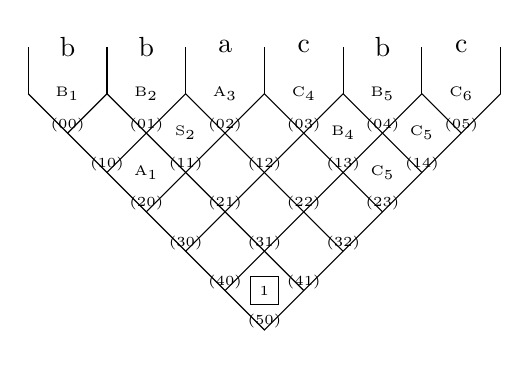
\begin{tikzpicture}[baseline]
			\newcommand{\myfontvars}[1]{
				\fontsize{4.9}{12}\selectfont{#1}
			}\newcommand{\myfontnumbering}[1]{
				\fontsize{2.5}{12}\selectfont{#1}
			}%Outer hull
			%Tip of the pyramid
			\coordinate (tip) at (3.0,-3.0);
			\foreach \i in {0,...,6} {
				\coordinate (\i) at (\i,0);
			}
			%Draw the left and right line of the pyramid pointing downwards
			\draw (0) -- (tip) -- (6);
			%Grid lines direction down-left to top-right
			\coordinate (dl1) at (0.5,-0.5);
			\coordinate (dl2) at (1.0,-1.0);
			\coordinate (dl3) at (1.5,-1.5);
			\coordinate (dl4) at (2.0,-2.0);
			\coordinate (dl5) at (2.5,-2.5);
			\draw (dl1) -- (1,0);
			\draw (dl2) -- (2,0);
			\draw (dl3) -- (3,0);
			\draw (dl4) -- (4,0);
			\draw (dl5) -- (5,0);
			%Grid lines direction down-right to top-left
			\coordinate (dr1) at (3.5,-2.5);
			\coordinate (dr2) at (4.0,-2.0);
			\coordinate (dr3) at (4.5,-1.5);
			\coordinate (dr4) at (5.0,-1.0);
			\coordinate (dr5) at (5.5,-0.5);
			\draw (dr1) -- (1,0);
			\draw (dr2) -- (2,0);
			\draw (dr3) -- (3,0);
			\draw (dr4) -- (4,0);
			\draw (dr5) -- (5,0);
			%Small lines at the top
			\coordinate (top0) at (0.0,0.0);
			\coordinate (top1) at (1.0,0.0);
			\coordinate (top2) at (2.0,0.0);
			\coordinate (top3) at (3.0,0.0);
			\coordinate (top4) at (4.0,0.0);
			\coordinate (top5) at (5.0,0.0);
			\coordinate (top6) at (6.0,0.0);
			\coordinate (topUpper0) at (0.0,0.6);
			\coordinate (topUpper1) at (1.0,0.6);
			\coordinate (topUpper2) at (2.0,0.6);
			\coordinate (topUpper3) at (3.0,0.6);
			\coordinate (topUpper4) at (4.0,0.6);
			\coordinate (topUpper5) at (5.0,0.6);
			\coordinate (topUpper6) at (6.0,0.6);
			\draw (top0) -- (topUpper0);
			\draw (top1) -- (topUpper1);
			\draw (top2) -- (topUpper2);
			\draw (top3) -- (topUpper3);
			\draw (top4) -- (topUpper4);
			\draw (top5) -- (topUpper5);
			\draw (top6) -- (topUpper6);
			%The string
			\coordinate (w0) at (0.5,0.6);
			\coordinate (w1) at (1.5,0.6);
			\coordinate (w2) at (2.5,0.6);
			\coordinate (w3) at (3.5,0.6);
			\coordinate (w4) at (4.5,0.6);
			\coordinate (w5) at (5.5,0.6);
			\node [] at (w0) {b};
			\node [] at (w1) {b};
			\node [] at (w2) {a};
			\node [] at (w3) {c};
			\node [] at (w4) {b};
			\node [] at (w5) {c};
			% Variables in the cells
			%cells00
			\coordinate (center00) at (0.5,0.0);
			\node [below=0.18cm] at (center00) {\myfontnumbering{$(00)$}};
			\node [] at (center00) {\myfontvars{B$_{1}$}};
			%cells01
			\coordinate (center01) at (1.5,0.0);
			\node [below=0.18cm] at (center01) {\myfontnumbering{$(01)$}};
			\node [] at (center01) {\myfontvars{B$_{2}$}};
			%cells02
			\coordinate (center02) at (2.5,0.0);
			\node [below=0.18cm] at (center02) {\myfontnumbering{$(02)$}};
			\node [] at (center02) {\myfontvars{A$_{3}$}};
			%cells03
			\coordinate (center03) at (3.5,0.0);
			\node [below=0.18cm] at (center03) {\myfontnumbering{$(03)$}};
			\node [] at (center03) {\myfontvars{C$_{4}$}};
			%cells04
			\coordinate (center04) at (4.5,0.0);
			\node [below=0.18cm] at (center04) {\myfontnumbering{$(04)$}};
			\node [] at (center04) {\myfontvars{B$_{5}$}};
			%cells05
			\coordinate (center05) at (5.5,0.0);
			\node [below=0.18cm] at (center05) {\myfontnumbering{$(05)$}};
			\node [] at (center05) {\myfontvars{C$_{6}$}};
			%cells10
			\coordinate (center10) at (1.0,-0.5);
			\node [below=0.18cm] at (center10) {\myfontnumbering{$(10)$}};
			%cells11
			\coordinate (center11) at (2.0,-0.5);
			\node [below=0.18cm] at (center11) {\myfontnumbering{$(11)$}};
			\node [] at (center11) {\myfontvars{S$_{2}$}};
			%cells12
			\coordinate (center12) at (3.0,-0.5);
			\node [below=0.18cm] at (center12) {\myfontnumbering{$(12)$}};
			%cells13
			\coordinate (center13) at (4.0,-0.5);
			\node [below=0.18cm] at (center13) {\myfontnumbering{$(13)$}};
			\node [] at (center13) {\myfontvars{B$_{4}$}};
			%cells14
			\coordinate (center14) at (5.0,-0.5);
			\node [below=0.18cm] at (center14) {\myfontnumbering{$(14)$}};
			\node [] at (center14) {\myfontvars{C$_{5}$}};
			%cells20
			\coordinate (center20) at (1.5,-1.0);
			\node [below=0.18cm] at (center20) {\myfontnumbering{$(20)$}};
			\node [] at (center20) {\myfontvars{A$_{1}$}};
			%cells21
			\coordinate (center21) at (2.5,-1.0);
			\node [below=0.18cm] at (center21) {\myfontnumbering{$(21)$}};
			%cells22
			\coordinate (center22) at (3.5,-1.0);
			\node [below=0.18cm] at (center22) {\myfontnumbering{$(22)$}};
			%cells23
			\coordinate (center23) at (4.5,-1.0);
			\node [below=0.18cm] at (center23) {\myfontnumbering{$(23)$}};
			\node [] at (center23) {\myfontvars{C$_{5}$}};
			%cells30
			\coordinate (center30) at (2.0,-1.5);
			\node [below=0.18cm] at (center30) {\myfontnumbering{$(30)$}};
			%cells31
			\coordinate (center31) at (3.0,-1.5);
			\node [below=0.18cm] at (center31) {\myfontnumbering{$(31)$}};
			%cells32
			\coordinate (center32) at (4.0,-1.5);
			\node [below=0.18cm] at (center32) {\myfontnumbering{$(32)$}};
			%cells40
			\coordinate (center40) at (2.5,-2.0);
			\node [below=0.18cm] at (center40) {\myfontnumbering{$(40)$}};
			%cells41
			\coordinate (center41) at (3.5,-2.0);
			\node [below=0.18cm] at (center41) {\myfontnumbering{$(41)$}};
			%cells50
			\coordinate (center50) at (3.0,-2.5);
			\node [below=0.18cm] at (center50) {\myfontnumbering{$(50)$}};
			\node [] at (center50) [minimum height=0.25cm,minimum width=0.25cm,draw] {\tiny{1}};
			\end{tikzpicture}
		}
	\end{minipage}
	\caption{Illustration of Algorithm \ref{SplitThenFill} part 5. Recursion step in $Cell_{2,3}$ is  resolved by adding the rule $C\rightarrow BC$.}
	\label{IllustrationAlgorithmSplitThenFillPart5}
\end{figure}
\noindent
\begin{figure} [h]
	\begin{minipage}{6in}
		\centering
		\begin{tabular}{l}
			$A\rightarrow B S~|~a~~$\\ 
			$B\rightarrow C B~|~b$\\ 
			$C\rightarrow B C~|~ c$\\ 
			$S\rightarrow B A~|~A C~~$\\ 
		\end{tabular}
		\resizebox{0.7\linewidth}{!}{
			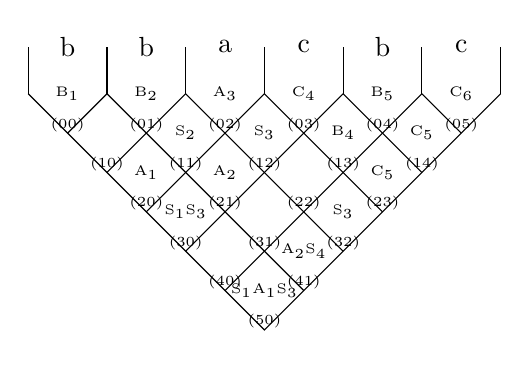
\begin{tikzpicture}[baseline]
			\newcommand{\myfontvars}[1]{
				\fontsize{4.9}{12}\selectfont{#1}
			}\newcommand{\myfontnumbering}[1]{
				\fontsize{2.5}{12}\selectfont{#1}
			}%Outer hull
			%Tip of the pyramid
			\coordinate (tip) at (3.0,-3.0);
			\foreach \i in {0,...,6} {
				\coordinate (\i) at (\i,0);
			}
			%Draw the left and right line of the pyramid pointing downwards
			\draw (0) -- (tip) -- (6);
			%Grid lines direction down-left to top-right
			\coordinate (dl1) at (0.5,-0.5);
			\coordinate (dl2) at (1.0,-1.0);
			\coordinate (dl3) at (1.5,-1.5);
			\coordinate (dl4) at (2.0,-2.0);
			\coordinate (dl5) at (2.5,-2.5);
			\draw (dl1) -- (1,0);
			\draw (dl2) -- (2,0);
			\draw (dl3) -- (3,0);
			\draw (dl4) -- (4,0);
			\draw (dl5) -- (5,0);
			%Grid lines direction down-right to top-left
			\coordinate (dr1) at (3.5,-2.5);
			\coordinate (dr2) at (4.0,-2.0);
			\coordinate (dr3) at (4.5,-1.5);
			\coordinate (dr4) at (5.0,-1.0);
			\coordinate (dr5) at (5.5,-0.5);
			\draw (dr1) -- (1,0);
			\draw (dr2) -- (2,0);
			\draw (dr3) -- (3,0);
			\draw (dr4) -- (4,0);
			\draw (dr5) -- (5,0);
			%Small lines at the top
			\coordinate (top0) at (0.0,0.0);
			\coordinate (top1) at (1.0,0.0);
			\coordinate (top2) at (2.0,0.0);
			\coordinate (top3) at (3.0,0.0);
			\coordinate (top4) at (4.0,0.0);
			\coordinate (top5) at (5.0,0.0);
			\coordinate (top6) at (6.0,0.0);
			\coordinate (topUpper0) at (0.0,0.6);
			\coordinate (topUpper1) at (1.0,0.6);
			\coordinate (topUpper2) at (2.0,0.6);
			\coordinate (topUpper3) at (3.0,0.6);
			\coordinate (topUpper4) at (4.0,0.6);
			\coordinate (topUpper5) at (5.0,0.6);
			\coordinate (topUpper6) at (6.0,0.6);
			\draw (top0) -- (topUpper0);
			\draw (top1) -- (topUpper1);
			\draw (top2) -- (topUpper2);
			\draw (top3) -- (topUpper3);
			\draw (top4) -- (topUpper4);
			\draw (top5) -- (topUpper5);
			\draw (top6) -- (topUpper6);
			%The string
			\coordinate (w0) at (0.5,0.6);
			\coordinate (w1) at (1.5,0.6);
			\coordinate (w2) at (2.5,0.6);
			\coordinate (w3) at (3.5,0.6);
			\coordinate (w4) at (4.5,0.6);
			\coordinate (w5) at (5.5,0.6);
			\node [] at (w0) {b};
			\node [] at (w1) {b};
			\node [] at (w2) {a};
			\node [] at (w3) {c};
			\node [] at (w4) {b};
			\node [] at (w5) {c};
			% Variables in the cells
			%cells00
			\coordinate (center00) at (0.5,0.0);
			\node [below=0.18cm] at (center00) {\myfontnumbering{$(00)$}};
			\node [] at (center00) {\myfontvars{B$_{1}$}};
			%cells01
			\coordinate (center01) at (1.5,0.0);
			\node [below=0.18cm] at (center01) {\myfontnumbering{$(01)$}};
			\node [] at (center01) {\myfontvars{B$_{2}$}};
			%cells02
			\coordinate (center02) at (2.5,0.0);
			\node [below=0.18cm] at (center02) {\myfontnumbering{$(02)$}};
			\node [] at (center02) {\myfontvars{A$_{3}$}};
			%cells03
			\coordinate (center03) at (3.5,0.0);
			\node [below=0.18cm] at (center03) {\myfontnumbering{$(03)$}};
			\node [] at (center03) {\myfontvars{C$_{4}$}};
			%cells04
			\coordinate (center04) at (4.5,0.0);
			\node [below=0.18cm] at (center04) {\myfontnumbering{$(04)$}};
			\node [] at (center04) {\myfontvars{B$_{5}$}};
			%cells05
			\coordinate (center05) at (5.5,0.0);
			\node [below=0.18cm] at (center05) {\myfontnumbering{$(05)$}};
			\node [] at (center05) {\myfontvars{C$_{6}$}};
			%cells10
			\coordinate (center10) at (1.0,-0.5);
			\node [below=0.18cm] at (center10) {\myfontnumbering{$(10)$}};
			%cells11
			\coordinate (center11) at (2.0,-0.5);
			\node [below=0.18cm] at (center11) {\myfontnumbering{$(11)$}};
			\node [] at (center11) {\myfontvars{S$_{2}$}};
			%cells12
			\coordinate (center12) at (3.0,-0.5);
			\node [below=0.18cm] at (center12) {\myfontnumbering{$(12)$}};
			\node [] at (center12) {\myfontvars{S$_{3}$}};
			%cells13
			\coordinate (center13) at (4.0,-0.5);
			\node [below=0.18cm] at (center13) {\myfontnumbering{$(13)$}};
			\node [] at (center13) {\myfontvars{B$_{4}$}};
			%cells14
			\coordinate (center14) at (5.0,-0.5);
			\node [below=0.18cm] at (center14) {\myfontnumbering{$(14)$}};
			\node [] at (center14) {\myfontvars{C$_{5}$}};
			%cells20
			\coordinate (center20) at (1.5,-1.0);
			\node [below=0.18cm] at (center20) {\myfontnumbering{$(20)$}};
			\node [] at (center20) {\myfontvars{A$_{1}$}};
			%cells21
			\coordinate (center21) at (2.5,-1.0);
			\node [below=0.18cm] at (center21) {\myfontnumbering{$(21)$}};
			\node [] at (center21) {\myfontvars{A$_{2}$}};
			%cells22
			\coordinate (center22) at (3.5,-1.0);
			\node [below=0.18cm] at (center22) {\myfontnumbering{$(22)$}};
			%cells23
			\coordinate (center23) at (4.5,-1.0);
			\node [below=0.18cm] at (center23) {\myfontnumbering{$(23)$}};
			\node [] at (center23) {\myfontvars{C$_{5}$}};
			%cells30
			\coordinate (center30) at (2.0,-1.5);
			\node [below=0.18cm] at (center30) {\myfontnumbering{$(30)$}};
			\node [] at (center30) {\myfontvars{S$_{1}$S$_{3}$}};
			%cells31
			\coordinate (center31) at (3.0,-1.5);
			\node [below=0.18cm] at (center31) {\myfontnumbering{$(31)$}};
			%cells32
			\coordinate (center32) at (4.0,-1.5);
			\node [below=0.18cm] at (center32) {\myfontnumbering{$(32)$}};
			\node [] at (center32) {\myfontvars{S$_{3}$}};
			%cells40
			\coordinate (center40) at (2.5,-2.0);
			\node [below=0.18cm] at (center40) {\myfontnumbering{$(40)$}};
			%cells41
			\coordinate (center41) at (3.5,-2.0);
			\node [below=0.18cm] at (center41) {\myfontnumbering{$(41)$}};
			\node [] at (center41) {\myfontvars{A$_{2}$S$_{4}$}};
			%cells50
			\coordinate (center50) at (3.0,-2.5);
			\node [below=0.18cm] at (center50) {\myfontnumbering{$(50)$}};
			\node [] at (center50) {\myfontvars{S$_{1}$A$_{1}$S$_{3}$}};
			\end{tikzpicture}
		}
	\end{minipage}
	\caption{Illustration of Algorithm \ref{SplitThenFill} part 6. Recursion step in $Cell_{5,0}$ is  resolved by adding the rule $S\rightarrow AC$.}
	\label{IllustrationAlgorithmSplitThenFillPart6}
\end{figure}\\

\clearpage

\subsection{SplitAndFill}
Algorithm \ref{SplitThenFill} creates the derivation tree structure Top-Downwards but adds rules to the grammar Bottom-Upwards. Another way to do this would be an attempt to do both Top-Downwards.\\
This algorithm therefore makes use of a part of the same idea as Algorithm \ref{SplitThenFill}. It also uses the concept of generating a predefined structure of the derivation tree Top-Downwards. The difference now is, that every time a node of the structure of the derivation tree has been decided on a rule is directly added to the grammar \textendash~therefore the name SplitAndFill, which is like "split for a node and then directly add a rule so that the node is then filled with at least one variable". \\
Note that the count of rules in the grammar is dependent on the count of nodes in the derivation tree and a terminal is distributed to only one variable. Further while resolving the last recursion step (Line \ref{splitAndFillRecLastStep}) of Algorithm \ref{SplitAndFillRecursion} the start variable will be in the tip in the pyramid that always leads to $w \in L(G)$.\\

\noindent
\frame{
	\begin{algorithm}[H] %or another one check
		\caption{SplitAndFill}
		\label{SplitAndFill}
		\SetAlgoLined
		\KwIn{Word $w \in \Sigma^{*}$}
		\KwOut{Set of productions $P$}
		$P = \emptyset$;~~\tcp{$P \subseteq V \times (V^{2} \cup \Sigma)$}
		$Sol = (P_{Sol},~v)$;~~\tcp{$P_{Sol} \subseteq P$} \label{cell}
		$Sol = SplitAndFillRec(P,\ w,\ i_{max},\ 0)$\;
		\Return $P_{Sol}$\;
				\footnotetext{
			\noindent Note: $v$ is a random element $v\in V$.
		}
	\end{algorithm}
}\\

\noindent
\frame{
	\begin{algorithm}[H] %or another one check
		\caption{SplitAndFillRec}
		\label{SplitAndFillRecursion}
		\SetAlgoLined
		\KwIn{$P_{in} \subseteq V \times (V^{2} \cup \Sigma),\ w \in \Sigma^{*},\ i,j \in \mathbb{N}$ }
		\KwOut{$(P,~v)$}
		$P = P_{in}$\;
		\If{$i=0$}{
			\If{terminal $w_j$ not distributed yet}{
				\Return $(P \cup \{(v,~ w_j)\},\ v_{lhse})$\;	
			}
			\Return $(P,\ v_{lhse})$\;	
		}
		$choose\ one\ m\ uniform\ randomly\ in\ [j+1,\ j+i]$\;
		$(P,\ v_l) = SplitAndFillRec(P,\ w,\ (m-j-1),\ j)$\label{left}\;
		$(P,\ v_r) = SplitAndFillRec(P,\ w,\ (j+i-m),\ m)$\label{right}\;	
		\If{$i=i_{max}$}{
			\Return $(P \cup \{(S,~v_l v_r)\},\ S)$\; \label{splitAndFillRecLastStep}
		}
		\Return $(P \cup \{(v,~v_l v_r)\},\ v)$\;
		\footnotetext{
			\noindent Note to $v$: $v$ is a random element $v\in V$.\\
			\noindent Note to $v_{lhse}$: There is the rule $v_{lhse}\rightarrow w_j$, i.e. $v_{lhse}$ is the variable on the left side of the one rule that has the terminal as its rhse.
		}
	\end{algorithm}
}
\\
Looking at this algorithm only productions according to the tree structure are added to the grammar. For illustration purposes now, the pyramid here is also shown to reflect the immediate changes of the added rules to the pyramid. Again the predefined derivation tree structure of Figure \ref{treeStruct} is used. Starting point is always a empty grammar.
\noindent
\begin{figure} [h]
	\begin{minipage}{6in}
		\centering
		\begin{tabular}{l}
			Grammar:\\
			$A \rightarrow $\\
			$B \rightarrow b$\\ 
			$C \rightarrow $\\
			$S \rightarrow $\\ 
		\end{tabular} 
		\resizebox{0.65\linewidth}{!}{
		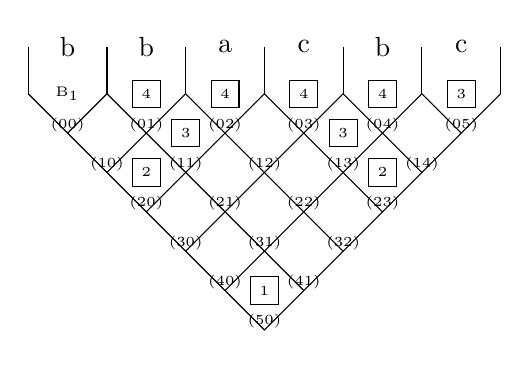
\begin{tikzpicture}[baseline]
		\newcommand{\myfontvars}[1]{
			\fontsize{4.9}{12}\selectfont{#1}
		}\newcommand{\myfontnumbering}[1]{
			\fontsize{2.5}{12}\selectfont{#1}
		}%Outer hull
		%Tip of the pyramid
		\coordinate (tip) at (3.0,-3.0);
		\foreach \i in {0,...,6} {
			\coordinate (\i) at (\i,0);
		}
		%Draw the left and right line of the pyramid pointing downwards
		\draw (0) -- (tip) -- (6);
		%Grid lines direction down-left to top-right
		\coordinate (dl1) at (0.5,-0.5);
		\coordinate (dl2) at (1.0,-1.0);
		\coordinate (dl3) at (1.5,-1.5);
		\coordinate (dl4) at (2.0,-2.0);
		\coordinate (dl5) at (2.5,-2.5);
		\draw (dl1) -- (1,0);
		\draw (dl2) -- (2,0);
		\draw (dl3) -- (3,0);
		\draw (dl4) -- (4,0);
		\draw (dl5) -- (5,0);
		%Grid lines direction down-right to top-left
		\coordinate (dr1) at (3.5,-2.5);
		\coordinate (dr2) at (4.0,-2.0);
		\coordinate (dr3) at (4.5,-1.5);
		\coordinate (dr4) at (5.0,-1.0);
		\coordinate (dr5) at (5.5,-0.5);
		\draw (dr1) -- (1,0);
		\draw (dr2) -- (2,0);
		\draw (dr3) -- (3,0);
		\draw (dr4) -- (4,0);
		\draw (dr5) -- (5,0);
		%Small lines at the top
		\coordinate (top0) at (0.0,0.0);
		\coordinate (top1) at (1.0,0.0);
		\coordinate (top2) at (2.0,0.0);
		\coordinate (top3) at (3.0,0.0);
		\coordinate (top4) at (4.0,0.0);
		\coordinate (top5) at (5.0,0.0);
		\coordinate (top6) at (6.0,0.0);
		\coordinate (topUpper0) at (0.0,0.6);
		\coordinate (topUpper1) at (1.0,0.6);
		\coordinate (topUpper2) at (2.0,0.6);
		\coordinate (topUpper3) at (3.0,0.6);
		\coordinate (topUpper4) at (4.0,0.6);
		\coordinate (topUpper5) at (5.0,0.6);
		\coordinate (topUpper6) at (6.0,0.6);
		\draw (top0) -- (topUpper0);
		\draw (top1) -- (topUpper1);
		\draw (top2) -- (topUpper2);
		\draw (top3) -- (topUpper3);
		\draw (top4) -- (topUpper4);
		\draw (top5) -- (topUpper5);
		\draw (top6) -- (topUpper6);
		%The string
		\coordinate (w0) at (0.5,0.6);
		\coordinate (w1) at (1.5,0.6);
		\coordinate (w2) at (2.5,0.6);
		\coordinate (w3) at (3.5,0.6);
		\coordinate (w4) at (4.5,0.6);
		\coordinate (w5) at (5.5,0.6);
		\node [] at (w0) {b};
		\node [] at (w1) {b};
		\node [] at (w2) {a};
		\node [] at (w3) {c};
		\node [] at (w4) {b};
		\node [] at (w5) {c};
		% Variables in the cells
		%cells00
		\coordinate (center00) at (0.5,0.0);
		\node [below=0.18cm] at (center00) {\myfontnumbering{$(00)$}};
		\node [] at (center00) {\myfontvars{B$_{1}$}};
		%cells01
		\coordinate (center01) at (1.5,0.0);
		\node [below=0.18cm] at (center01) {\myfontnumbering{$(01)$}};
		\node [] at (center01) [minimum height=0.25cm,minimum width=0.25cm,draw] {\tiny{4}};
		%cells02
		\coordinate (center02) at (2.5,0.0);
		\node [below=0.18cm] at (center02) {\myfontnumbering{$(02)$}};
		\node [] at (center02) [minimum height=0.25cm,minimum width=0.25cm,draw] {\tiny{4}};
		%cells03
		\coordinate (center03) at (3.5,0.0);
		\node [below=0.18cm] at (center03) {\myfontnumbering{$(03)$}};
		\node [] at (center03) [minimum height=0.25cm,minimum width=0.25cm,draw] {\tiny{4}};
		%cells04
		\coordinate (center04) at (4.5,0.0);
		\node [below=0.18cm] at (center04) {\myfontnumbering{$(04)$}};
		\node [] at (center04) [minimum height=0.25cm,minimum width=0.25cm,draw] {\tiny{4}};
		%cells05
		\coordinate (center05) at (5.5,0.0);
		\node [below=0.18cm] at (center05) {\myfontnumbering{$(05)$}};
		\node [] at (center05) [minimum height=0.25cm,minimum width=0.25cm,draw] {\tiny{3}};
		%cells10
		\coordinate (center10) at (1.0,-0.5);
		\node [below=0.18cm] at (center10) {\myfontnumbering{$(10)$}};
		%cells11
		\coordinate (center11) at (2.0,-0.5);
		\node [below=0.18cm] at (center11) {\myfontnumbering{$(11)$}};
		\node [] at (center11) [minimum height=0.25cm,minimum width=0.25cm,draw] {\tiny{3}};
		%cells12
		\coordinate (center12) at (3.0,-0.5);
		\node [below=0.18cm] at (center12) {\myfontnumbering{$(12)$}};
		%cells13
		\coordinate (center13) at (4.0,-0.5);
		\node [below=0.18cm] at (center13) {\myfontnumbering{$(13)$}};
		\node [] at (center13) [minimum height=0.25cm,minimum width=0.25cm,draw] {\tiny{3}};
		%cells14
		\coordinate (center14) at (5.0,-0.5);
		\node [below=0.18cm] at (center14) {\myfontnumbering{$(14)$}};
		%cells20
		\coordinate (center20) at (1.5,-1.0);
		\node [below=0.18cm] at (center20) {\myfontnumbering{$(20)$}};
		\node [] at (center20) [minimum height=0.25cm,minimum width=0.25cm,draw] {\tiny{2}};
		%cells21
		\coordinate (center21) at (2.5,-1.0);
		\node [below=0.18cm] at (center21) {\myfontnumbering{$(21)$}};
		%cells22
		\coordinate (center22) at (3.5,-1.0);
		\node [below=0.18cm] at (center22) {\myfontnumbering{$(22)$}};
		%cells23
		\coordinate (center23) at (4.5,-1.0);
		\node [below=0.18cm] at (center23) {\myfontnumbering{$(23)$}};
		\node [] at (center23) [minimum height=0.25cm,minimum width=0.25cm,draw] {\tiny{2}};
		%cells30
		\coordinate (center30) at (2.0,-1.5);
		\node [below=0.18cm] at (center30) {\myfontnumbering{$(30)$}};
		%cells31
		\coordinate (center31) at (3.0,-1.5);
		\node [below=0.18cm] at (center31) {\myfontnumbering{$(31)$}};
		%cells32
		\coordinate (center32) at (4.0,-1.5);
		\node [below=0.18cm] at (center32) {\myfontnumbering{$(32)$}};
		%cells40
		\coordinate (center40) at (2.5,-2.0);
		\node [below=0.18cm] at (center40) {\myfontnumbering{$(40)$}};
		%cells41
		\coordinate (center41) at (3.5,-2.0);
		\node [below=0.18cm] at (center41) {\myfontnumbering{$(41)$}};
		%cells50
		\coordinate (center50) at (3.0,-2.5);
		\node [below=0.18cm] at (center50) {\myfontnumbering{$(50)$}};
		\node [] at (center50) [minimum height=0.25cm,minimum width=0.25cm,draw] {\tiny{1}};
		\end{tikzpicture}
	}
	\end{minipage}
	\caption{Illustration of Algorithm \ref{SplitAndFill} part 1. To resolve the recursion step that fills $Cell_{0,0}$ the rule $B\rightarrow b$ is added.}
	\label{IllustrationAlgorithmSplitAndFillPart1}
\end{figure}

\noindent
\begin{figure} [h]
	\begin{minipage}{6in}
		\centering
		\begin{tabular}{l}
			Grammar:\\
			$A \rightarrow a$\\
			$B \rightarrow b$\\ 
			$C \rightarrow $\\
			$S \rightarrow BA$\\ 
		\end{tabular} 
		\resizebox{0.65\linewidth}{!}{
			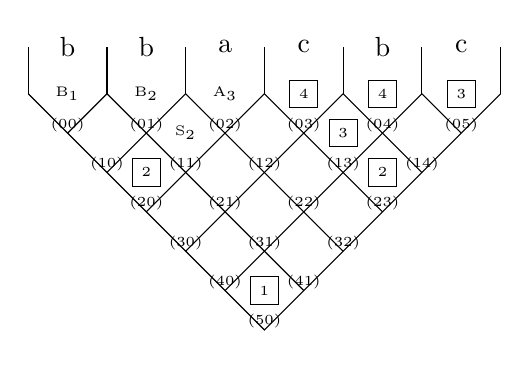
\begin{tikzpicture}[baseline]
			\newcommand{\myfontvars}[1]{
				\fontsize{4.9}{12}\selectfont{#1}
			}\newcommand{\myfontnumbering}[1]{
				\fontsize{2.5}{12}\selectfont{#1}
			}%Outer hull
			%Tip of the pyramid
			\coordinate (tip) at (3.0,-3.0);
			\foreach \i in {0,...,6} {
				\coordinate (\i) at (\i,0);
			}
			%Draw the left and right line of the pyramid pointing downwards
			\draw (0) -- (tip) -- (6);
			%Grid lines direction down-left to top-right
			\coordinate (dl1) at (0.5,-0.5);
			\coordinate (dl2) at (1.0,-1.0);
			\coordinate (dl3) at (1.5,-1.5);
			\coordinate (dl4) at (2.0,-2.0);
			\coordinate (dl5) at (2.5,-2.5);
			\draw (dl1) -- (1,0);
			\draw (dl2) -- (2,0);
			\draw (dl3) -- (3,0);
			\draw (dl4) -- (4,0);
			\draw (dl5) -- (5,0);
			%Grid lines direction down-right to top-left
			\coordinate (dr1) at (3.5,-2.5);
			\coordinate (dr2) at (4.0,-2.0);
			\coordinate (dr3) at (4.5,-1.5);
			\coordinate (dr4) at (5.0,-1.0);
			\coordinate (dr5) at (5.5,-0.5);
			\draw (dr1) -- (1,0);
			\draw (dr2) -- (2,0);
			\draw (dr3) -- (3,0);
			\draw (dr4) -- (4,0);
			\draw (dr5) -- (5,0);
			%Small lines at the top
			\coordinate (top0) at (0.0,0.0);
			\coordinate (top1) at (1.0,0.0);
			\coordinate (top2) at (2.0,0.0);
			\coordinate (top3) at (3.0,0.0);
			\coordinate (top4) at (4.0,0.0);
			\coordinate (top5) at (5.0,0.0);
			\coordinate (top6) at (6.0,0.0);
			\coordinate (topUpper0) at (0.0,0.6);
			\coordinate (topUpper1) at (1.0,0.6);
			\coordinate (topUpper2) at (2.0,0.6);
			\coordinate (topUpper3) at (3.0,0.6);
			\coordinate (topUpper4) at (4.0,0.6);
			\coordinate (topUpper5) at (5.0,0.6);
			\coordinate (topUpper6) at (6.0,0.6);
			\draw (top0) -- (topUpper0);
			\draw (top1) -- (topUpper1);
			\draw (top2) -- (topUpper2);
			\draw (top3) -- (topUpper3);
			\draw (top4) -- (topUpper4);
			\draw (top5) -- (topUpper5);
			\draw (top6) -- (topUpper6);
			%The string
			\coordinate (w0) at (0.5,0.6);
			\coordinate (w1) at (1.5,0.6);
			\coordinate (w2) at (2.5,0.6);
			\coordinate (w3) at (3.5,0.6);
			\coordinate (w4) at (4.5,0.6);
			\coordinate (w5) at (5.5,0.6);
			\node [] at (w0) {b};
			\node [] at (w1) {b};
			\node [] at (w2) {a};
			\node [] at (w3) {c};
			\node [] at (w4) {b};
			\node [] at (w5) {c};
			% Variables in the cells
			%cells00
			\coordinate (center00) at (0.5,0.0);
			\node [below=0.18cm] at (center00) {\myfontnumbering{$(00)$}};
			\node [] at (center00) {\myfontvars{B$_{1}$}};
			%cells01
			\coordinate (center01) at (1.5,0.0);
			\node [below=0.18cm] at (center01) {\myfontnumbering{$(01)$}};
			\node [] at (center01) {\myfontvars{B$_{2}$}};
			%cells02
			\coordinate (center02) at (2.5,0.0);
			\node [below=0.18cm] at (center02) {\myfontnumbering{$(02)$}};
			\node [] at (center02) {\myfontvars{A$_{3}$}};
			%cells03
			\coordinate (center03) at (3.5,0.0);
			\node [below=0.18cm] at (center03) {\myfontnumbering{$(03)$}};
			\node [] at (center03) [minimum height=0.25cm,minimum width=0.25cm,draw] {\tiny{4}};
			%cells04
			\coordinate (center04) at (4.5,0.0);
			\node [below=0.18cm] at (center04) {\myfontnumbering{$(04)$}};
			\node [] at (center04) [minimum height=0.25cm,minimum width=0.25cm,draw] {\tiny{4}};
			%cells05
			\coordinate (center05) at (5.5,0.0);
			\node [below=0.18cm] at (center05) {\myfontnumbering{$(05)$}};
			\node [] at (center05) [minimum height=0.25cm,minimum width=0.25cm,draw] {\tiny{3}};
			%cells10
			\coordinate (center10) at (1.0,-0.5);
			\node [below=0.18cm] at (center10) {\myfontnumbering{$(10)$}};
			%cells11
			\coordinate (center11) at (2.0,-0.5);
			\node [below=0.18cm] at (center11) {\myfontnumbering{$(11)$}};
			\node [] at (center11) {\myfontvars{S$_{2}$}};
			%cells12
			\coordinate (center12) at (3.0,-0.5);
			\node [below=0.18cm] at (center12) {\myfontnumbering{$(12)$}};
			%cells13
			\coordinate (center13) at (4.0,-0.5);
			\node [below=0.18cm] at (center13) {\myfontnumbering{$(13)$}};
			\node [] at (center13) [minimum height=0.25cm,minimum width=0.25cm,draw] {\tiny{3}};
			%cells14
			\coordinate (center14) at (5.0,-0.5);
			\node [below=0.18cm] at (center14) {\myfontnumbering{$(14)$}};
			%cells20
			\coordinate (center20) at (1.5,-1.0);
			\node [below=0.18cm] at (center20) {\myfontnumbering{$(20)$}};
			\node [] at (center20) [minimum height=0.25cm,minimum width=0.25cm,draw] {\tiny{2}};
			%cells21
			\coordinate (center21) at (2.5,-1.0);
			\node [below=0.18cm] at (center21) {\myfontnumbering{$(21)$}};
			%cells22
			\coordinate (center22) at (3.5,-1.0);
			\node [below=0.18cm] at (center22) {\myfontnumbering{$(22)$}};
			%cells23
			\coordinate (center23) at (4.5,-1.0);
			\node [below=0.18cm] at (center23) {\myfontnumbering{$(23)$}};
			\node [] at (center23) [minimum height=0.25cm,minimum width=0.25cm,draw] {\tiny{2}};
			%cells30
			\coordinate (center30) at (2.0,-1.5);
			\node [below=0.18cm] at (center30) {\myfontnumbering{$(30)$}};
			%cells31
			\coordinate (center31) at (3.0,-1.5);
			\node [below=0.18cm] at (center31) {\myfontnumbering{$(31)$}};
			%cells32
			\coordinate (center32) at (4.0,-1.5);
			\node [below=0.18cm] at (center32) {\myfontnumbering{$(32)$}};
			%cells40
			\coordinate (center40) at (2.5,-2.0);
			\node [below=0.18cm] at (center40) {\myfontnumbering{$(40)$}};
			%cells41
			\coordinate (center41) at (3.5,-2.0);
			\node [below=0.18cm] at (center41) {\myfontnumbering{$(41)$}};
			%cells50
			\coordinate (center50) at (3.0,-2.5);
			\node [below=0.18cm] at (center50) {\myfontnumbering{$(50)$}};
			\node [] at (center50) [minimum height=0.25cm,minimum width=0.25cm,draw] {\tiny{1}};
			\end{tikzpicture}
		}
	\end{minipage}
	\caption{Illustration of Algorithm \ref{SplitAndFill} part 2. Resolving the recursion step that fills $Cell_{0,1}$ no rule is added because a rule $lhse\rightarrow b$ already exists. To fill $Cell_{0,2}$ the rule $A\rightarrow a$ is added. Regarding $Cell_{1,1}$ the rule $S \rightarrow BA$ is added.}
	\label{IllustrationAlgorithmSplitAndFillPart2}
\end{figure}
\noindent
\begin{figure} [h]
	\begin{minipage}{6in}
		\centering
		\begin{tabular}{l}
			Grammar:\\
			$A \rightarrow a$\\
			$B \rightarrow b$\\ 
			$C \rightarrow BS$\\
			$S \rightarrow BA$\\ 
		\end{tabular} 
		\resizebox{0.65\linewidth}{!}{
			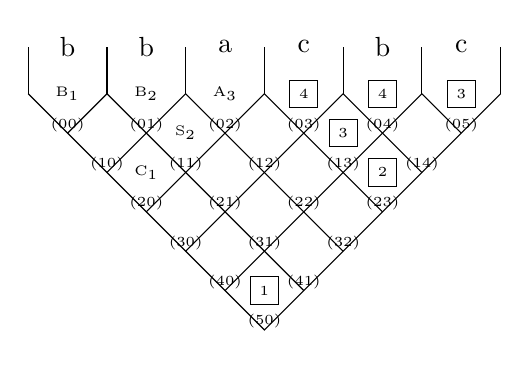
\begin{tikzpicture}[baseline]
			\newcommand{\myfontvars}[1]{
				\fontsize{4.9}{12}\selectfont{#1}
			}\newcommand{\myfontnumbering}[1]{
				\fontsize{2.5}{12}\selectfont{#1}
			}%Outer hull
			%Tip of the pyramid
			\coordinate (tip) at (3.0,-3.0);
			\foreach \i in {0,...,6} {
				\coordinate (\i) at (\i,0);
			}
			%Draw the left and right line of the pyramid pointing downwards
			\draw (0) -- (tip) -- (6);
			%Grid lines direction down-left to top-right
			\coordinate (dl1) at (0.5,-0.5);
			\coordinate (dl2) at (1.0,-1.0);
			\coordinate (dl3) at (1.5,-1.5);
			\coordinate (dl4) at (2.0,-2.0);
			\coordinate (dl5) at (2.5,-2.5);
			\draw (dl1) -- (1,0);
			\draw (dl2) -- (2,0);
			\draw (dl3) -- (3,0);
			\draw (dl4) -- (4,0);
			\draw (dl5) -- (5,0);
			%Grid lines direction down-right to top-left
			\coordinate (dr1) at (3.5,-2.5);
			\coordinate (dr2) at (4.0,-2.0);
			\coordinate (dr3) at (4.5,-1.5);
			\coordinate (dr4) at (5.0,-1.0);
			\coordinate (dr5) at (5.5,-0.5);
			\draw (dr1) -- (1,0);
			\draw (dr2) -- (2,0);
			\draw (dr3) -- (3,0);
			\draw (dr4) -- (4,0);
			\draw (dr5) -- (5,0);
			%Small lines at the top
			\coordinate (top0) at (0.0,0.0);
			\coordinate (top1) at (1.0,0.0);
			\coordinate (top2) at (2.0,0.0);
			\coordinate (top3) at (3.0,0.0);
			\coordinate (top4) at (4.0,0.0);
			\coordinate (top5) at (5.0,0.0);
			\coordinate (top6) at (6.0,0.0);
			\coordinate (topUpper0) at (0.0,0.6);
			\coordinate (topUpper1) at (1.0,0.6);
			\coordinate (topUpper2) at (2.0,0.6);
			\coordinate (topUpper3) at (3.0,0.6);
			\coordinate (topUpper4) at (4.0,0.6);
			\coordinate (topUpper5) at (5.0,0.6);
			\coordinate (topUpper6) at (6.0,0.6);
			\draw (top0) -- (topUpper0);
			\draw (top1) -- (topUpper1);
			\draw (top2) -- (topUpper2);
			\draw (top3) -- (topUpper3);
			\draw (top4) -- (topUpper4);
			\draw (top5) -- (topUpper5);
			\draw (top6) -- (topUpper6);
			%The string
			\coordinate (w0) at (0.5,0.6);
			\coordinate (w1) at (1.5,0.6);
			\coordinate (w2) at (2.5,0.6);
			\coordinate (w3) at (3.5,0.6);
			\coordinate (w4) at (4.5,0.6);
			\coordinate (w5) at (5.5,0.6);
			\node [] at (w0) {b};
			\node [] at (w1) {b};
			\node [] at (w2) {a};
			\node [] at (w3) {c};
			\node [] at (w4) {b};
			\node [] at (w5) {c};
			% Variables in the cells
			%cells00
			\coordinate (center00) at (0.5,0.0);
			\node [below=0.18cm] at (center00) {\myfontnumbering{$(00)$}};
			\node [] at (center00) {\myfontvars{B$_{1}$}};
			%cells01
			\coordinate (center01) at (1.5,0.0);
			\node [below=0.18cm] at (center01) {\myfontnumbering{$(01)$}};
			\node [] at (center01) {\myfontvars{B$_{2}$}};
			%cells02
			\coordinate (center02) at (2.5,0.0);
			\node [below=0.18cm] at (center02) {\myfontnumbering{$(02)$}};
			\node [] at (center02) {\myfontvars{A$_{3}$}};
			%cells03
			\coordinate (center03) at (3.5,0.0);
			\node [below=0.18cm] at (center03) {\myfontnumbering{$(03)$}};
			\node [] at (center03) [minimum height=0.25cm,minimum width=0.25cm,draw] {\tiny{4}};
			%cells04
			\coordinate (center04) at (4.5,0.0);
			\node [below=0.18cm] at (center04) {\myfontnumbering{$(04)$}};
			\node [] at (center04) [minimum height=0.25cm,minimum width=0.25cm,draw] {\tiny{4}};
			%cells05
			\coordinate (center05) at (5.5,0.0);
			\node [below=0.18cm] at (center05) {\myfontnumbering{$(05)$}};
			\node [] at (center05) [minimum height=0.25cm,minimum width=0.25cm,draw] {\tiny{3}};
			%cells10
			\coordinate (center10) at (1.0,-0.5);
			\node [below=0.18cm] at (center10) {\myfontnumbering{$(10)$}};
			%cells11
			\coordinate (center11) at (2.0,-0.5);
			\node [below=0.18cm] at (center11) {\myfontnumbering{$(11)$}};
			\node [] at (center11) {\myfontvars{S$_{2}$}};
			%cells12
			\coordinate (center12) at (3.0,-0.5);
			\node [below=0.18cm] at (center12) {\myfontnumbering{$(12)$}};
			%cells13
			\coordinate (center13) at (4.0,-0.5);
			\node [below=0.18cm] at (center13) {\myfontnumbering{$(13)$}};
			\node [] at (center13) [minimum height=0.25cm,minimum width=0.25cm,draw] {\tiny{3}};
			%cells14
			\coordinate (center14) at (5.0,-0.5);
			\node [below=0.18cm] at (center14) {\myfontnumbering{$(14)$}};
			%cells20
			\coordinate (center20) at (1.5,-1.0);
			\node [below=0.18cm] at (center20) {\myfontnumbering{$(20)$}};
			\node [] at (center20) {\myfontvars{C$_{1}$}};
			%cells21
			\coordinate (center21) at (2.5,-1.0);
			\node [below=0.18cm] at (center21) {\myfontnumbering{$(21)$}};
			%cells22
			\coordinate (center22) at (3.5,-1.0);
			\node [below=0.18cm] at (center22) {\myfontnumbering{$(22)$}};
			%cells23
			\coordinate (center23) at (4.5,-1.0);
			\node [below=0.18cm] at (center23) {\myfontnumbering{$(23)$}};
			\node [] at (center23) [minimum height=0.25cm,minimum width=0.25cm,draw] {\tiny{2}};
			%cells30
			\coordinate (center30) at (2.0,-1.5);
			\node [below=0.18cm] at (center30) {\myfontnumbering{$(30)$}};
			%cells31
			\coordinate (center31) at (3.0,-1.5);
			\node [below=0.18cm] at (center31) {\myfontnumbering{$(31)$}};
			%cells32
			\coordinate (center32) at (4.0,-1.5);
			\node [below=0.18cm] at (center32) {\myfontnumbering{$(32)$}};
			%cells40
			\coordinate (center40) at (2.5,-2.0);
			\node [below=0.18cm] at (center40) {\myfontnumbering{$(40)$}};
			%cells41
			\coordinate (center41) at (3.5,-2.0);
			\node [below=0.18cm] at (center41) {\myfontnumbering{$(41)$}};
			%cells50
			\coordinate (center50) at (3.0,-2.5);
			\node [below=0.18cm] at (center50) {\myfontnumbering{$(50)$}};
			\node [] at (center50) [minimum height=0.25cm,minimum width=0.25cm,draw] {\tiny{1}};
			\end{tikzpicture}
		}
	\end{minipage}
	\caption{Illustration of Algorithm \ref{SplitAndFill} part 3. Filling the $Cell_{2,0}$ the rule $C \rightarrow BS$ is added.}
	\label{IllustrationAlgorithmSplitAndFillPart3}
\end{figure}
\noindent
\begin{figure} [h]
	\begin{minipage}{6in}
		\centering
		\begin{tabular}{l}
			Grammar:\\
			$A \rightarrow BC~|~a$\\
			$B \rightarrow CB~|~b$\\ 
			$C \rightarrow BS~|~c$\\
			$S \rightarrow BA$\\ 
		\end{tabular} 
		\resizebox{0.65\linewidth}{!}{
			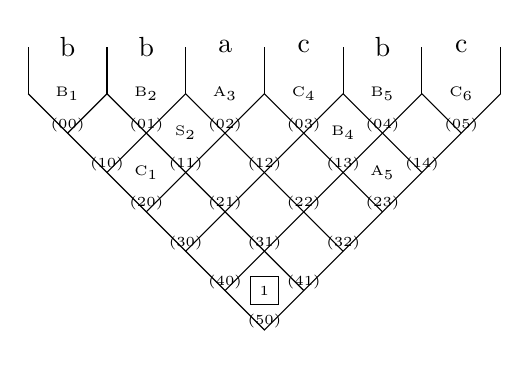
\begin{tikzpicture}[baseline]
			\newcommand{\myfontvars}[1]{
				\fontsize{4.9}{12}\selectfont{#1}
			}\newcommand{\myfontnumbering}[1]{
				\fontsize{2.5}{12}\selectfont{#1}
			}%Outer hull
			%Tip of the pyramid
			\coordinate (tip) at (3.0,-3.0);
			\foreach \i in {0,...,6} {
				\coordinate (\i) at (\i,0);
			}
			%Draw the left and right line of the pyramid pointing downwards
			\draw (0) -- (tip) -- (6);
			%Grid lines direction down-left to top-right
			\coordinate (dl1) at (0.5,-0.5);
			\coordinate (dl2) at (1.0,-1.0);
			\coordinate (dl3) at (1.5,-1.5);
			\coordinate (dl4) at (2.0,-2.0);
			\coordinate (dl5) at (2.5,-2.5);
			\draw (dl1) -- (1,0);
			\draw (dl2) -- (2,0);
			\draw (dl3) -- (3,0);
			\draw (dl4) -- (4,0);
			\draw (dl5) -- (5,0);
			%Grid lines direction down-right to top-left
			\coordinate (dr1) at (3.5,-2.5);
			\coordinate (dr2) at (4.0,-2.0);
			\coordinate (dr3) at (4.5,-1.5);
			\coordinate (dr4) at (5.0,-1.0);
			\coordinate (dr5) at (5.5,-0.5);
			\draw (dr1) -- (1,0);
			\draw (dr2) -- (2,0);
			\draw (dr3) -- (3,0);
			\draw (dr4) -- (4,0);
			\draw (dr5) -- (5,0);
			%Small lines at the top
			\coordinate (top0) at (0.0,0.0);
			\coordinate (top1) at (1.0,0.0);
			\coordinate (top2) at (2.0,0.0);
			\coordinate (top3) at (3.0,0.0);
			\coordinate (top4) at (4.0,0.0);
			\coordinate (top5) at (5.0,0.0);
			\coordinate (top6) at (6.0,0.0);
			\coordinate (topUpper0) at (0.0,0.6);
			\coordinate (topUpper1) at (1.0,0.6);
			\coordinate (topUpper2) at (2.0,0.6);
			\coordinate (topUpper3) at (3.0,0.6);
			\coordinate (topUpper4) at (4.0,0.6);
			\coordinate (topUpper5) at (5.0,0.6);
			\coordinate (topUpper6) at (6.0,0.6);
			\draw (top0) -- (topUpper0);
			\draw (top1) -- (topUpper1);
			\draw (top2) -- (topUpper2);
			\draw (top3) -- (topUpper3);
			\draw (top4) -- (topUpper4);
			\draw (top5) -- (topUpper5);
			\draw (top6) -- (topUpper6);
			%The string
			\coordinate (w0) at (0.5,0.6);
			\coordinate (w1) at (1.5,0.6);
			\coordinate (w2) at (2.5,0.6);
			\coordinate (w3) at (3.5,0.6);
			\coordinate (w4) at (4.5,0.6);
			\coordinate (w5) at (5.5,0.6);
			\node [] at (w0) {b};
			\node [] at (w1) {b};
			\node [] at (w2) {a};
			\node [] at (w3) {c};
			\node [] at (w4) {b};
			\node [] at (w5) {c};
			% Variables in the cells
			%cells00
			\coordinate (center00) at (0.5,0.0);
			\node [below=0.18cm] at (center00) {\myfontnumbering{$(00)$}};
			\node [] at (center00) {\myfontvars{B$_{1}$}};
			%cells01
			\coordinate (center01) at (1.5,0.0);
			\node [below=0.18cm] at (center01) {\myfontnumbering{$(01)$}};
			\node [] at (center01) {\myfontvars{B$_{2}$}};
			%cells02
			\coordinate (center02) at (2.5,0.0);
			\node [below=0.18cm] at (center02) {\myfontnumbering{$(02)$}};
			\node [] at (center02) {\myfontvars{A$_{3}$}};
			%cells03
			\coordinate (center03) at (3.5,0.0);
			\node [below=0.18cm] at (center03) {\myfontnumbering{$(03)$}};
			\node [] at (center03) {\myfontvars{C$_{4}$}};
			%cells04
			\coordinate (center04) at (4.5,0.0);
			\node [below=0.18cm] at (center04) {\myfontnumbering{$(04)$}};
			\node [] at (center04) {\myfontvars{B$_{5}$}};
			%cells05
			\coordinate (center05) at (5.5,0.0);
			\node [below=0.18cm] at (center05) {\myfontnumbering{$(05)$}};
			\node [] at (center05) {\myfontvars{C$_{6}$}};
			%cells10
			\coordinate (center10) at (1.0,-0.5);
			\node [below=0.18cm] at (center10) {\myfontnumbering{$(10)$}};
			%cells11
			\coordinate (center11) at (2.0,-0.5);
			\node [below=0.18cm] at (center11) {\myfontnumbering{$(11)$}};
			\node [] at (center11) {\myfontvars{S$_{2}$}};
			%cells12
			\coordinate (center12) at (3.0,-0.5);
			\node [below=0.18cm] at (center12) {\myfontnumbering{$(12)$}};
			%cells13
			\coordinate (center13) at (4.0,-0.5);
			\node [below=0.18cm] at (center13) {\myfontnumbering{$(13)$}};
			\node [] at (center13) {\myfontvars{B$_{4}$}};
			%cells14
			\coordinate (center14) at (5.0,-0.5);
			\node [below=0.18cm] at (center14) {\myfontnumbering{$(14)$}};
			%cells20
			\coordinate (center20) at (1.5,-1.0);
			\node [below=0.18cm] at (center20) {\myfontnumbering{$(20)$}};
			\node [] at (center20) {\myfontvars{C$_{1}$}};
			%cells21
			\coordinate (center21) at (2.5,-1.0);
			\node [below=0.18cm] at (center21) {\myfontnumbering{$(21)$}};
			%cells22
			\coordinate (center22) at (3.5,-1.0);
			\node [below=0.18cm] at (center22) {\myfontnumbering{$(22)$}};
			%cells23
			\coordinate (center23) at (4.5,-1.0);
			\node [below=0.18cm] at (center23) {\myfontnumbering{$(23)$}};
			\node [] at (center23) {\myfontvars{A$_{5}$}};
			%cells30
			\coordinate (center30) at (2.0,-1.5);
			\node [below=0.18cm] at (center30) {\myfontnumbering{$(30)$}};
			%cells31
			\coordinate (center31) at (3.0,-1.5);
			\node [below=0.18cm] at (center31) {\myfontnumbering{$(31)$}};
			%cells32
			\coordinate (center32) at (4.0,-1.5);
			\node [below=0.18cm] at (center32) {\myfontnumbering{$(32)$}};
			%cells40
			\coordinate (center40) at (2.5,-2.0);
			\node [below=0.18cm] at (center40) {\myfontnumbering{$(40)$}};
			%cells41
			\coordinate (center41) at (3.5,-2.0);
			\node [below=0.18cm] at (center41) {\myfontnumbering{$(41)$}};
			%cells50
			\coordinate (center50) at (3.0,-2.5);
			\node [below=0.18cm] at (center50) {\myfontnumbering{$(50)$}};
			\node [] at (center50) [minimum height=0.25cm,minimum width=0.25cm,draw] {\tiny{1}};
			\end{tikzpicture}
		}
	\end{minipage}
	\caption{Illustration of Algorithm \ref{SplitAndFill} part 4. In analogous manner the other cells are filled. $Cell_{03}$ is responsible for the rule $C \rightarrow c$, $Cell_{0,4}$ doesn't cause a rule because again there already is the rule $B \rightarrow b$, $Cell_{1,3}$ contributes for the rule $B \rightarrow CB$, $Cell_{0,5}$ doesn't add a rule because of $C\rightarrow c$ and to fill $Cell_{2,3}$ the rule $A \rightarrow BC$ is added.}
	\label{IllustrationAlgorithmSplitAndFillPart4}
\end{figure}

\noindent
\begin{figure} [h]
	\begin{minipage}{6in}
		\centering
		\begin{tabular}{l}
			Grammar:\\
			$A \rightarrow BC~|~a$\\
			$B \rightarrow CB~|~b$\\ 
			$C \rightarrow BS~|~c$\\
			$S \rightarrow BA~|~CA$\\ 
		\end{tabular} 
		\resizebox{0.65\linewidth}{!}{
			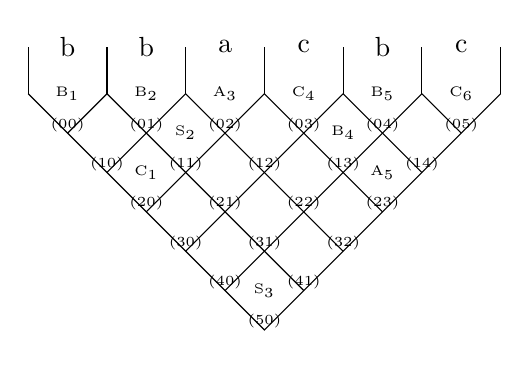
\begin{tikzpicture}[baseline]
			\newcommand{\myfontvars}[1]{
				\fontsize{4.9}{12}\selectfont{#1}
			}\newcommand{\myfontnumbering}[1]{
				\fontsize{2.5}{12}\selectfont{#1}
			}%Outer hull
			%Tip of the pyramid
			\coordinate (tip) at (3.0,-3.0);
			\foreach \i in {0,...,6} {
				\coordinate (\i) at (\i,0);
			}
			%Draw the left and right line of the pyramid pointing downwards
			\draw (0) -- (tip) -- (6);
			%Grid lines direction down-left to top-right
			\coordinate (dl1) at (0.5,-0.5);
			\coordinate (dl2) at (1.0,-1.0);
			\coordinate (dl3) at (1.5,-1.5);
			\coordinate (dl4) at (2.0,-2.0);
			\coordinate (dl5) at (2.5,-2.5);
			\draw (dl1) -- (1,0);
			\draw (dl2) -- (2,0);
			\draw (dl3) -- (3,0);
			\draw (dl4) -- (4,0);
			\draw (dl5) -- (5,0);
			%Grid lines direction down-right to top-left
			\coordinate (dr1) at (3.5,-2.5);
			\coordinate (dr2) at (4.0,-2.0);
			\coordinate (dr3) at (4.5,-1.5);
			\coordinate (dr4) at (5.0,-1.0);
			\coordinate (dr5) at (5.5,-0.5);
			\draw (dr1) -- (1,0);
			\draw (dr2) -- (2,0);
			\draw (dr3) -- (3,0);
			\draw (dr4) -- (4,0);
			\draw (dr5) -- (5,0);
			%Small lines at the top
			\coordinate (top0) at (0.0,0.0);
			\coordinate (top1) at (1.0,0.0);
			\coordinate (top2) at (2.0,0.0);
			\coordinate (top3) at (3.0,0.0);
			\coordinate (top4) at (4.0,0.0);
			\coordinate (top5) at (5.0,0.0);
			\coordinate (top6) at (6.0,0.0);
			\coordinate (topUpper0) at (0.0,0.6);
			\coordinate (topUpper1) at (1.0,0.6);
			\coordinate (topUpper2) at (2.0,0.6);
			\coordinate (topUpper3) at (3.0,0.6);
			\coordinate (topUpper4) at (4.0,0.6);
			\coordinate (topUpper5) at (5.0,0.6);
			\coordinate (topUpper6) at (6.0,0.6);
			\draw (top0) -- (topUpper0);
			\draw (top1) -- (topUpper1);
			\draw (top2) -- (topUpper2);
			\draw (top3) -- (topUpper3);
			\draw (top4) -- (topUpper4);
			\draw (top5) -- (topUpper5);
			\draw (top6) -- (topUpper6);
			%The string
			\coordinate (w0) at (0.5,0.6);
			\coordinate (w1) at (1.5,0.6);
			\coordinate (w2) at (2.5,0.6);
			\coordinate (w3) at (3.5,0.6);
			\coordinate (w4) at (4.5,0.6);
			\coordinate (w5) at (5.5,0.6);
			\node [] at (w0) {b};
			\node [] at (w1) {b};
			\node [] at (w2) {a};
			\node [] at (w3) {c};
			\node [] at (w4) {b};
			\node [] at (w5) {c};
			% Variables in the cells
			%cells00
			\coordinate (center00) at (0.5,0.0);
			\node [below=0.18cm] at (center00) {\myfontnumbering{$(00)$}};
			\node [] at (center00) {\myfontvars{B$_{1}$}};
			%cells01
			\coordinate (center01) at (1.5,0.0);
			\node [below=0.18cm] at (center01) {\myfontnumbering{$(01)$}};
			\node [] at (center01) {\myfontvars{B$_{2}$}};
			%cells02
			\coordinate (center02) at (2.5,0.0);
			\node [below=0.18cm] at (center02) {\myfontnumbering{$(02)$}};
			\node [] at (center02) {\myfontvars{A$_{3}$}};
			%cells03
			\coordinate (center03) at (3.5,0.0);
			\node [below=0.18cm] at (center03) {\myfontnumbering{$(03)$}};
			\node [] at (center03) {\myfontvars{C$_{4}$}};
			%cells04
			\coordinate (center04) at (4.5,0.0);
			\node [below=0.18cm] at (center04) {\myfontnumbering{$(04)$}};
			\node [] at (center04) {\myfontvars{B$_{5}$}};
			%cells05
			\coordinate (center05) at (5.5,0.0);
			\node [below=0.18cm] at (center05) {\myfontnumbering{$(05)$}};
			\node [] at (center05) {\myfontvars{C$_{6}$}};
			%cells10
			\coordinate (center10) at (1.0,-0.5);
			\node [below=0.18cm] at (center10) {\myfontnumbering{$(10)$}};
			%cells11
			\coordinate (center11) at (2.0,-0.5);
			\node [below=0.18cm] at (center11) {\myfontnumbering{$(11)$}};
			\node [] at (center11) {\myfontvars{S$_{2}$}};
			%cells12
			\coordinate (center12) at (3.0,-0.5);
			\node [below=0.18cm] at (center12) {\myfontnumbering{$(12)$}};
			%cells13
			\coordinate (center13) at (4.0,-0.5);
			\node [below=0.18cm] at (center13) {\myfontnumbering{$(13)$}};
			\node [] at (center13) {\myfontvars{B$_{4}$}};
			%cells14
			\coordinate (center14) at (5.0,-0.5);
			\node [below=0.18cm] at (center14) {\myfontnumbering{$(14)$}};
			%cells20
			\coordinate (center20) at (1.5,-1.0);
			\node [below=0.18cm] at (center20) {\myfontnumbering{$(20)$}};
			\node [] at (center20) {\myfontvars{C$_{1}$}};
			%cells21
			\coordinate (center21) at (2.5,-1.0);
			\node [below=0.18cm] at (center21) {\myfontnumbering{$(21)$}};
			%cells22
			\coordinate (center22) at (3.5,-1.0);
			\node [below=0.18cm] at (center22) {\myfontnumbering{$(22)$}};
			%cells23
			\coordinate (center23) at (4.5,-1.0);
			\node [below=0.18cm] at (center23) {\myfontnumbering{$(23)$}};
			\node [] at (center23) {\myfontvars{A$_{5}$}};
			%cells30
			\coordinate (center30) at (2.0,-1.5);
			\node [below=0.18cm] at (center30) {\myfontnumbering{$(30)$}};
			%cells31
			\coordinate (center31) at (3.0,-1.5);
			\node [below=0.18cm] at (center31) {\myfontnumbering{$(31)$}};
			%cells32
			\coordinate (center32) at (4.0,-1.5);
			\node [below=0.18cm] at (center32) {\myfontnumbering{$(32)$}};
			%cells40
			\coordinate (center40) at (2.5,-2.0);
			\node [below=0.18cm] at (center40) {\myfontnumbering{$(40)$}};
			%cells41
			\coordinate (center41) at (3.5,-2.0);
			\node [below=0.18cm] at (center41) {\myfontnumbering{$(41)$}};
			%cells50
			\coordinate (center50) at (3.0,-2.5);
			\node [below=0.18cm] at (center50) {\myfontnumbering{$(50)$}};
			\node [] at (center50) {\myfontvars{S$_{3}$}};
			\end{tikzpicture}
		}
	\end{minipage}
	\caption{Illustration of Algorithm \ref{SplitAndFill} part 5. Finally to fill the cell in the tip a rule must be added that has the start variable as its $lhse$ that guarantees $w \in L(G)$. Here the rule $S\rightarrow CA$ is added.}
	\label{IllustrationAlgorithmSplitAndFillPart5}
\end{figure}

\noindent
\begin{figure} [h]
	\begin{minipage}{6in}
		\centering
		\begin{tabular}{l}
			Grammar:\\
			$A \rightarrow BC~|~a$\\
			$B \rightarrow CB~|~b$\\ 
			$C \rightarrow BS~|~c$\\
			$S \rightarrow BA~|~CA$\\ 
		\end{tabular} 
		\resizebox{0.65\linewidth}{!}{
			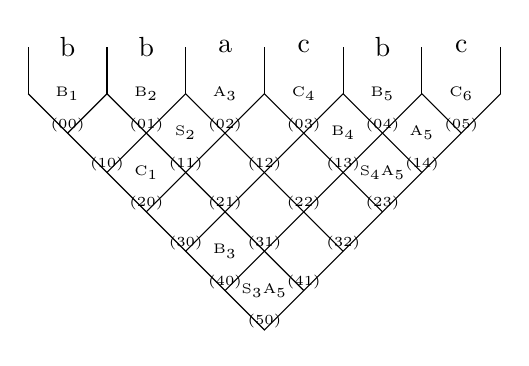
\begin{tikzpicture}[baseline]
			\newcommand{\myfontvars}[1]{
				\fontsize{4.9}{12}\selectfont{#1}
			}\newcommand{\myfontnumbering}[1]{
				\fontsize{2.5}{12}\selectfont{#1}
			}%Outer hull
			%Tip of the pyramid
			\coordinate (tip) at (3.0,-3.0);
			\foreach \i in {0,...,6} {
				\coordinate (\i) at (\i,0);
			}
			%Draw the left and right line of the pyramid pointing downwards
			\draw (0) -- (tip) -- (6);
			%Grid lines direction down-left to top-right
			\coordinate (dl1) at (0.5,-0.5);
			\coordinate (dl2) at (1.0,-1.0);
			\coordinate (dl3) at (1.5,-1.5);
			\coordinate (dl4) at (2.0,-2.0);
			\coordinate (dl5) at (2.5,-2.5);
			\draw (dl1) -- (1,0);
			\draw (dl2) -- (2,0);
			\draw (dl3) -- (3,0);
			\draw (dl4) -- (4,0);
			\draw (dl5) -- (5,0);
			%Grid lines direction down-right to top-left
			\coordinate (dr1) at (3.5,-2.5);
			\coordinate (dr2) at (4.0,-2.0);
			\coordinate (dr3) at (4.5,-1.5);
			\coordinate (dr4) at (5.0,-1.0);
			\coordinate (dr5) at (5.5,-0.5);
			\draw (dr1) -- (1,0);
			\draw (dr2) -- (2,0);
			\draw (dr3) -- (3,0);
			\draw (dr4) -- (4,0);
			\draw (dr5) -- (5,0);
			%Small lines at the top
			\coordinate (top0) at (0.0,0.0);
			\coordinate (top1) at (1.0,0.0);
			\coordinate (top2) at (2.0,0.0);
			\coordinate (top3) at (3.0,0.0);
			\coordinate (top4) at (4.0,0.0);
			\coordinate (top5) at (5.0,0.0);
			\coordinate (top6) at (6.0,0.0);
			\coordinate (topUpper0) at (0.0,0.6);
			\coordinate (topUpper1) at (1.0,0.6);
			\coordinate (topUpper2) at (2.0,0.6);
			\coordinate (topUpper3) at (3.0,0.6);
			\coordinate (topUpper4) at (4.0,0.6);
			\coordinate (topUpper5) at (5.0,0.6);
			\coordinate (topUpper6) at (6.0,0.6);
			\draw (top0) -- (topUpper0);
			\draw (top1) -- (topUpper1);
			\draw (top2) -- (topUpper2);
			\draw (top3) -- (topUpper3);
			\draw (top4) -- (topUpper4);
			\draw (top5) -- (topUpper5);
			\draw (top6) -- (topUpper6);
			%The string
			\coordinate (w0) at (0.5,0.6);
			\coordinate (w1) at (1.5,0.6);
			\coordinate (w2) at (2.5,0.6);
			\coordinate (w3) at (3.5,0.6);
			\coordinate (w4) at (4.5,0.6);
			\coordinate (w5) at (5.5,0.6);
			\node [] at (w0) {b};
			\node [] at (w1) {b};
			\node [] at (w2) {a};
			\node [] at (w3) {c};
			\node [] at (w4) {b};
			\node [] at (w5) {c};
			% Variables in the cells
			%cells00
			\coordinate (center00) at (0.5,0.0);
			\node [below=0.18cm] at (center00) {\myfontnumbering{$(00)$}};
			\node [] at (center00) {\myfontvars{B$_{1}$}};
			%cells01
			\coordinate (center01) at (1.5,0.0);
			\node [below=0.18cm] at (center01) {\myfontnumbering{$(01)$}};
			\node [] at (center01) {\myfontvars{B$_{2}$}};
			%cells02
			\coordinate (center02) at (2.5,0.0);
			\node [below=0.18cm] at (center02) {\myfontnumbering{$(02)$}};
			\node [] at (center02) {\myfontvars{A$_{3}$}};
			%cells03
			\coordinate (center03) at (3.5,0.0);
			\node [below=0.18cm] at (center03) {\myfontnumbering{$(03)$}};
			\node [] at (center03) {\myfontvars{C$_{4}$}};
			%cells04
			\coordinate (center04) at (4.5,0.0);
			\node [below=0.18cm] at (center04) {\myfontnumbering{$(04)$}};
			\node [] at (center04) {\myfontvars{B$_{5}$}};
			%cells05
			\coordinate (center05) at (5.5,0.0);
			\node [below=0.18cm] at (center05) {\myfontnumbering{$(05)$}};
			\node [] at (center05) {\myfontvars{C$_{6}$}};
			%cells10
			\coordinate (center10) at (1.0,-0.5);
			\node [below=0.18cm] at (center10) {\myfontnumbering{$(10)$}};
			%cells11
			\coordinate (center11) at (2.0,-0.5);
			\node [below=0.18cm] at (center11) {\myfontnumbering{$(11)$}};
			\node [] at (center11) {\myfontvars{S$_{2}$}};
			%cells12
			\coordinate (center12) at (3.0,-0.5);
			\node [below=0.18cm] at (center12) {\myfontnumbering{$(12)$}};
			%cells13
			\coordinate (center13) at (4.0,-0.5);
			\node [below=0.18cm] at (center13) {\myfontnumbering{$(13)$}};
			\node [] at (center13) {\myfontvars{B$_{4}$}};
			%cells14
			\coordinate (center14) at (5.0,-0.5);
			\node [below=0.18cm] at (center14) {\myfontnumbering{$(14)$}};
			\node [] at (center14) {\myfontvars{A$_{5}$}};
			%cells20
			\coordinate (center20) at (1.5,-1.0);
			\node [below=0.18cm] at (center20) {\myfontnumbering{$(20)$}};
			\node [] at (center20) {\myfontvars{C$_{1}$}};
			%cells21
			\coordinate (center21) at (2.5,-1.0);
			\node [below=0.18cm] at (center21) {\myfontnumbering{$(21)$}};
			%cells22
			\coordinate (center22) at (3.5,-1.0);
			\node [below=0.18cm] at (center22) {\myfontnumbering{$(22)$}};
			%cells23
			\coordinate (center23) at (4.5,-1.0);
			\node [below=0.18cm] at (center23) {\myfontnumbering{$(23)$}};
			\node [] at (center23) {\myfontvars{S$_{4}$A$_{5}$}};
			%cells30
			\coordinate (center30) at (2.0,-1.5);
			\node [below=0.18cm] at (center30) {\myfontnumbering{$(30)$}};
			%cells31
			\coordinate (center31) at (3.0,-1.5);
			\node [below=0.18cm] at (center31) {\myfontnumbering{$(31)$}};
			%cells32
			\coordinate (center32) at (4.0,-1.5);
			\node [below=0.18cm] at (center32) {\myfontnumbering{$(32)$}};
			%cells40
			\coordinate (center40) at (2.5,-2.0);
			\node [below=0.18cm] at (center40) {\myfontnumbering{$(40)$}};
			\node [] at (center40) {\myfontvars{B$_{3}$}};
			%cells41
			\coordinate (center41) at (3.5,-2.0);
			\node [below=0.18cm] at (center41) {\myfontnumbering{$(41)$}};
			%cells50
			\coordinate (center50) at (3.0,-2.5);
			\node [below=0.18cm] at (center50) {\myfontnumbering{$(50)$}};
			\node [] at (center50) {\myfontvars{S$_{3}$A$_{5}$}};
			\end{tikzpicture}
		}
	\end{minipage}
	\caption{Illustration of Algorithm \ref{SplitAndFill} part 6. With part 5 of the example the algorithm is finished. In comparison to Figure \ref{IllustrationAlgorithmSplitAndFillPart5} the complete parsing table looks like above.}
	\label{IllustrationAlgorithmSplitAndFillPart6}
\end{figure}

\clearpage
\pagebreak
\subsection{Comparision of Algorithms} \label{ComparisonOfAlgorithms}
\noindent Write about the standard configuration used.
\begin{table}[H]
	\centering
	\begin{tabular}{ | l | c |c |c |c | }
		\hline
Algorithm 		& SR 	& SR-Producibility 	& SR-Cardinality-Rules 	& SR-Pyramid   	\\ \hline
\hline
DiceRollOnly 	& 09~\%	& 24~\% & 88~\% & 39~\%		\\ \hline
BotomUpVar1 	& 16~\% & 52~\% & 90~\% & 41~\% 	\\ \hline
BotomUpVar2 	& 19~\% & 47~\% & 93~\% & 53~\% 	\\ \hline
SplitThenFill 	& 24~\% & 40~\% & 97~\% & 67~\% 	\\ \hline
SplitAndFill 	& 11~\% & 100~\% & 69~\% & 15~\% 	\\ \hline
	\end{tabular}
	\caption{Comparison of the SRs of the algorithms. Stopping criteria root not empty.}
	\label{comparisonAlgorithms}
\end{table}
Finding of ideal parameter for each algorithm.

\begin{table}[H]
	\centering
	\begin{tabular}{ | l | c |c |c |c | }
		\hline
		Algorithm 		& SR 	& SR-Producibility 	& SR-Cardinality-Rules 	& SR-Pyramid   	\\ \hline
		\hline
		DiceRollOnly 	& 09~\%	& 23~\% & 88~\% & 38~\%		\\ \hline
		BotomUpVar1 	& 11~\% & 30~\% & 99~\% & 58~\% 	\\ \hline
		BotomUpVar2 	& 13~\% & 26~\% & 99~\% & 66~\% 	\\ \hline
		SplitThenFill 	& 24~\% & 40~\% & 97~\% & 67~\% 	\\ \hline
		SplitAndFill 	& 11~\% & 100~\% & 70~\% & 14~\% 	\\ \hline
	\end{tabular}
	\caption{Comparison of the SRs of the algorithms. Stopping criteria more than half.}
	\label{comparisonAlgorithms}
\end{table}

Analysis of the problem space possibly visualized in heat maps.



\begin{table}[h]
	\centering
	\caption{My caption}
	\label{my-label}
	\begin{tabular}{|l|c|c|c|c|c|c|c|}
		\hline
		\multicolumn{1}{|c|}{Algorithm} & SR   & \begin{tabular}[c]{@{}c@{}}Produci-\\ bility\end{tabular} & \begin{tabular}[c]{@{}c@{}}Cardinality-\\ Rules\end{tabular} & \multicolumn{4}{c|}{Pyramid}                                                                                                                                                        \\ \cline{6-8} 
		&      &                                                           &                                                              &      & \begin{tabular}[c]{@{}c@{}}Force-\\ Right\end{tabular} & \begin{tabular}[c]{@{}c@{}}Vars-\\ PerCell\end{tabular} & \begin{tabular}[c]{@{}c@{}}VarsIn-\\ Pyramid\end{tabular} \\ \hline
		DiceRollOnly                    & 09\% &                                                           &                                                              & 67\% &                                                        &                                                         &                                                           \\ \hline
		BottomUpVar1                    &      &                                                           &                                                              &      &                                                        &                                                         &                                                           \\ \hline
		BottomUpVar2                    &      &                                                           &                                                              &      &                                                        &                                                         &                                                           \\ \hline
		SplitThenFill                   &      &                                                           &                                                              &      &                                                        &                                                         &                                                           \\ \hline
		SplitAndFill                    &      &                                                           &                                                              &      &                                                        &                                                         &                                                           \\ \hline
	\end{tabular}
\end{table}
\pagebreak